\documentclass{beamer}
\usepackage{multicol}

\usepackage{clrscode3e}
\usepackage{amsmath}
\usepackage{graphicx}

\newcommand{\bi}{\begin{itemize}}
\newcommand{\ii}{\item}
\newcommand{\ei}{\end{itemize}}
\newcommand{\bn}{\begin{enumerate}}
\newcommand{\en}{\end{enumerate}}
\newcommand{\set}[1]{\ensuremath{\left\{#1\right\}}}
\newcommand{\pr}[1]{\ensuremath{\mbox{Pr}\left\{#1\right\}}}
\newcommand{\flr}[1]{\ensuremath{\left\lfloor#1\right\rfloor}}
\newcommand{\ceil}[1]{\ensuremath{\left\lceil#1\right\rceil}}

\newcommand{\sect}[1]{
\section{#1}
\begin{frame}[fragile]\frametitle{#1}
}


\newcommand{\nop}[1]{}

\title{Notes on Binary Search Trees}
\author{Geoffrey Matthews}
\begin{document}
\begin{frame}
\maketitle
\end{frame}


\sect{Search Trees}
\bi
\ii Data structures that support many dynamic-set operations.
\ii Dictionaries and priority queues.
\ii Basic operations take time proportional to height of the tree.
\bi
\ii Best case: $\Theta(\lg n)$
\ii Worst case: $\Theta(n)$
\ei
\ii Different types of search trees:
\bi
\ii binary search trees
\ii red-black trees
\ii B-trees
\ei
\ii Only assume a comparison operator on keys.
\bi\ii Hash tables assume a key we can hash well.\ei
\ei

\end{frame}

\sect{Binary search trees}
\bi
\ii Many dynamic-set operations in $O(h)$ time, where $h = $ height of
tree. 
\ii We represent a binary tree by a linked data structure where each
node is an object.
\ii $T.root$ points to the root of the tree $T$.
\ii Each node contains the attributes:
\bi
\ii \textit{key} (and possibly other satellite data).
\ii \textit{left}: points to left child.
\ii \textit{right}: points to right child.
\ii \textit{p:} points to parent.  $T.root.p = $ \textsc{nil}
\ei
\ei

\end{frame}

\sect{Binary search tree property}
\bi
\ii If $y$ is in the left subtree of $x$, then $y.key \leq x.key$
\ii If $y$ is in the right subtree of $x$, then $y.key \geq x.key$
\ei
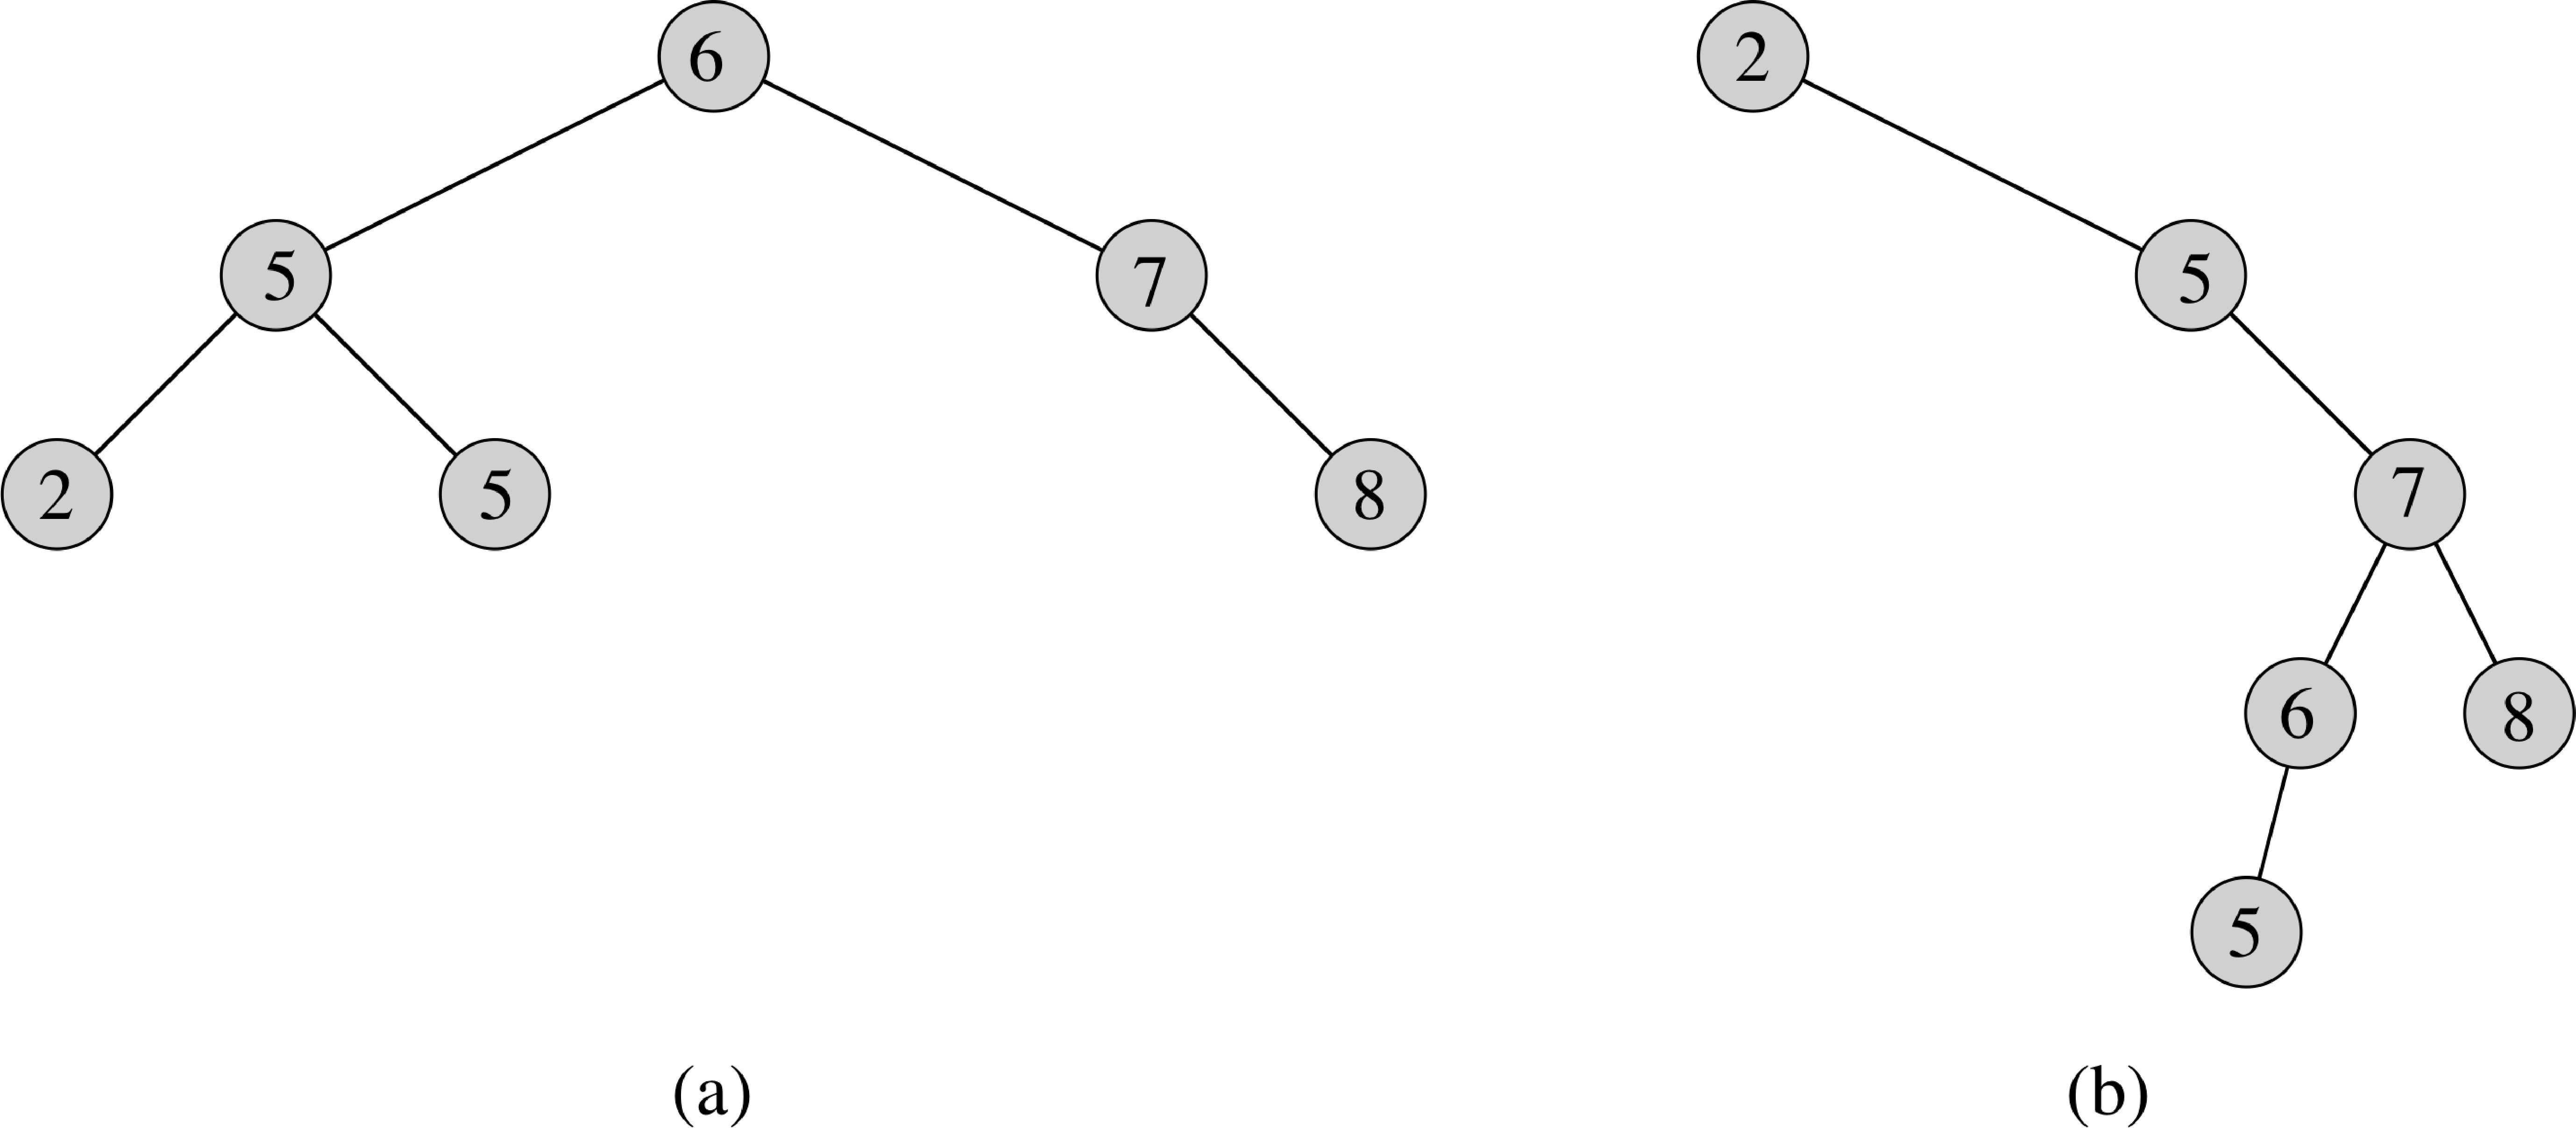
\includegraphics[width=\textwidth]{Fig-12-1.pdf}

\vfill

\bi\ii Frequently we assume keys are unique.\ei

\end{frame}
\sect{Inorder-Tree-Walk}

\begin{codebox}
  \Procname{$\proc{Inorder-Tree-Walk}(x)$}
  \li \If $x \not\isequal \const{nil}$ \Do
  \li $\proc{Inorder-Tree-Walk}(\attrib{x}{left})$
  \li print $\attrib{x}{key}$
  \li $\proc{Inorder-Tree-Walk}(\attrib{x}{right})$  
\end{codebox}

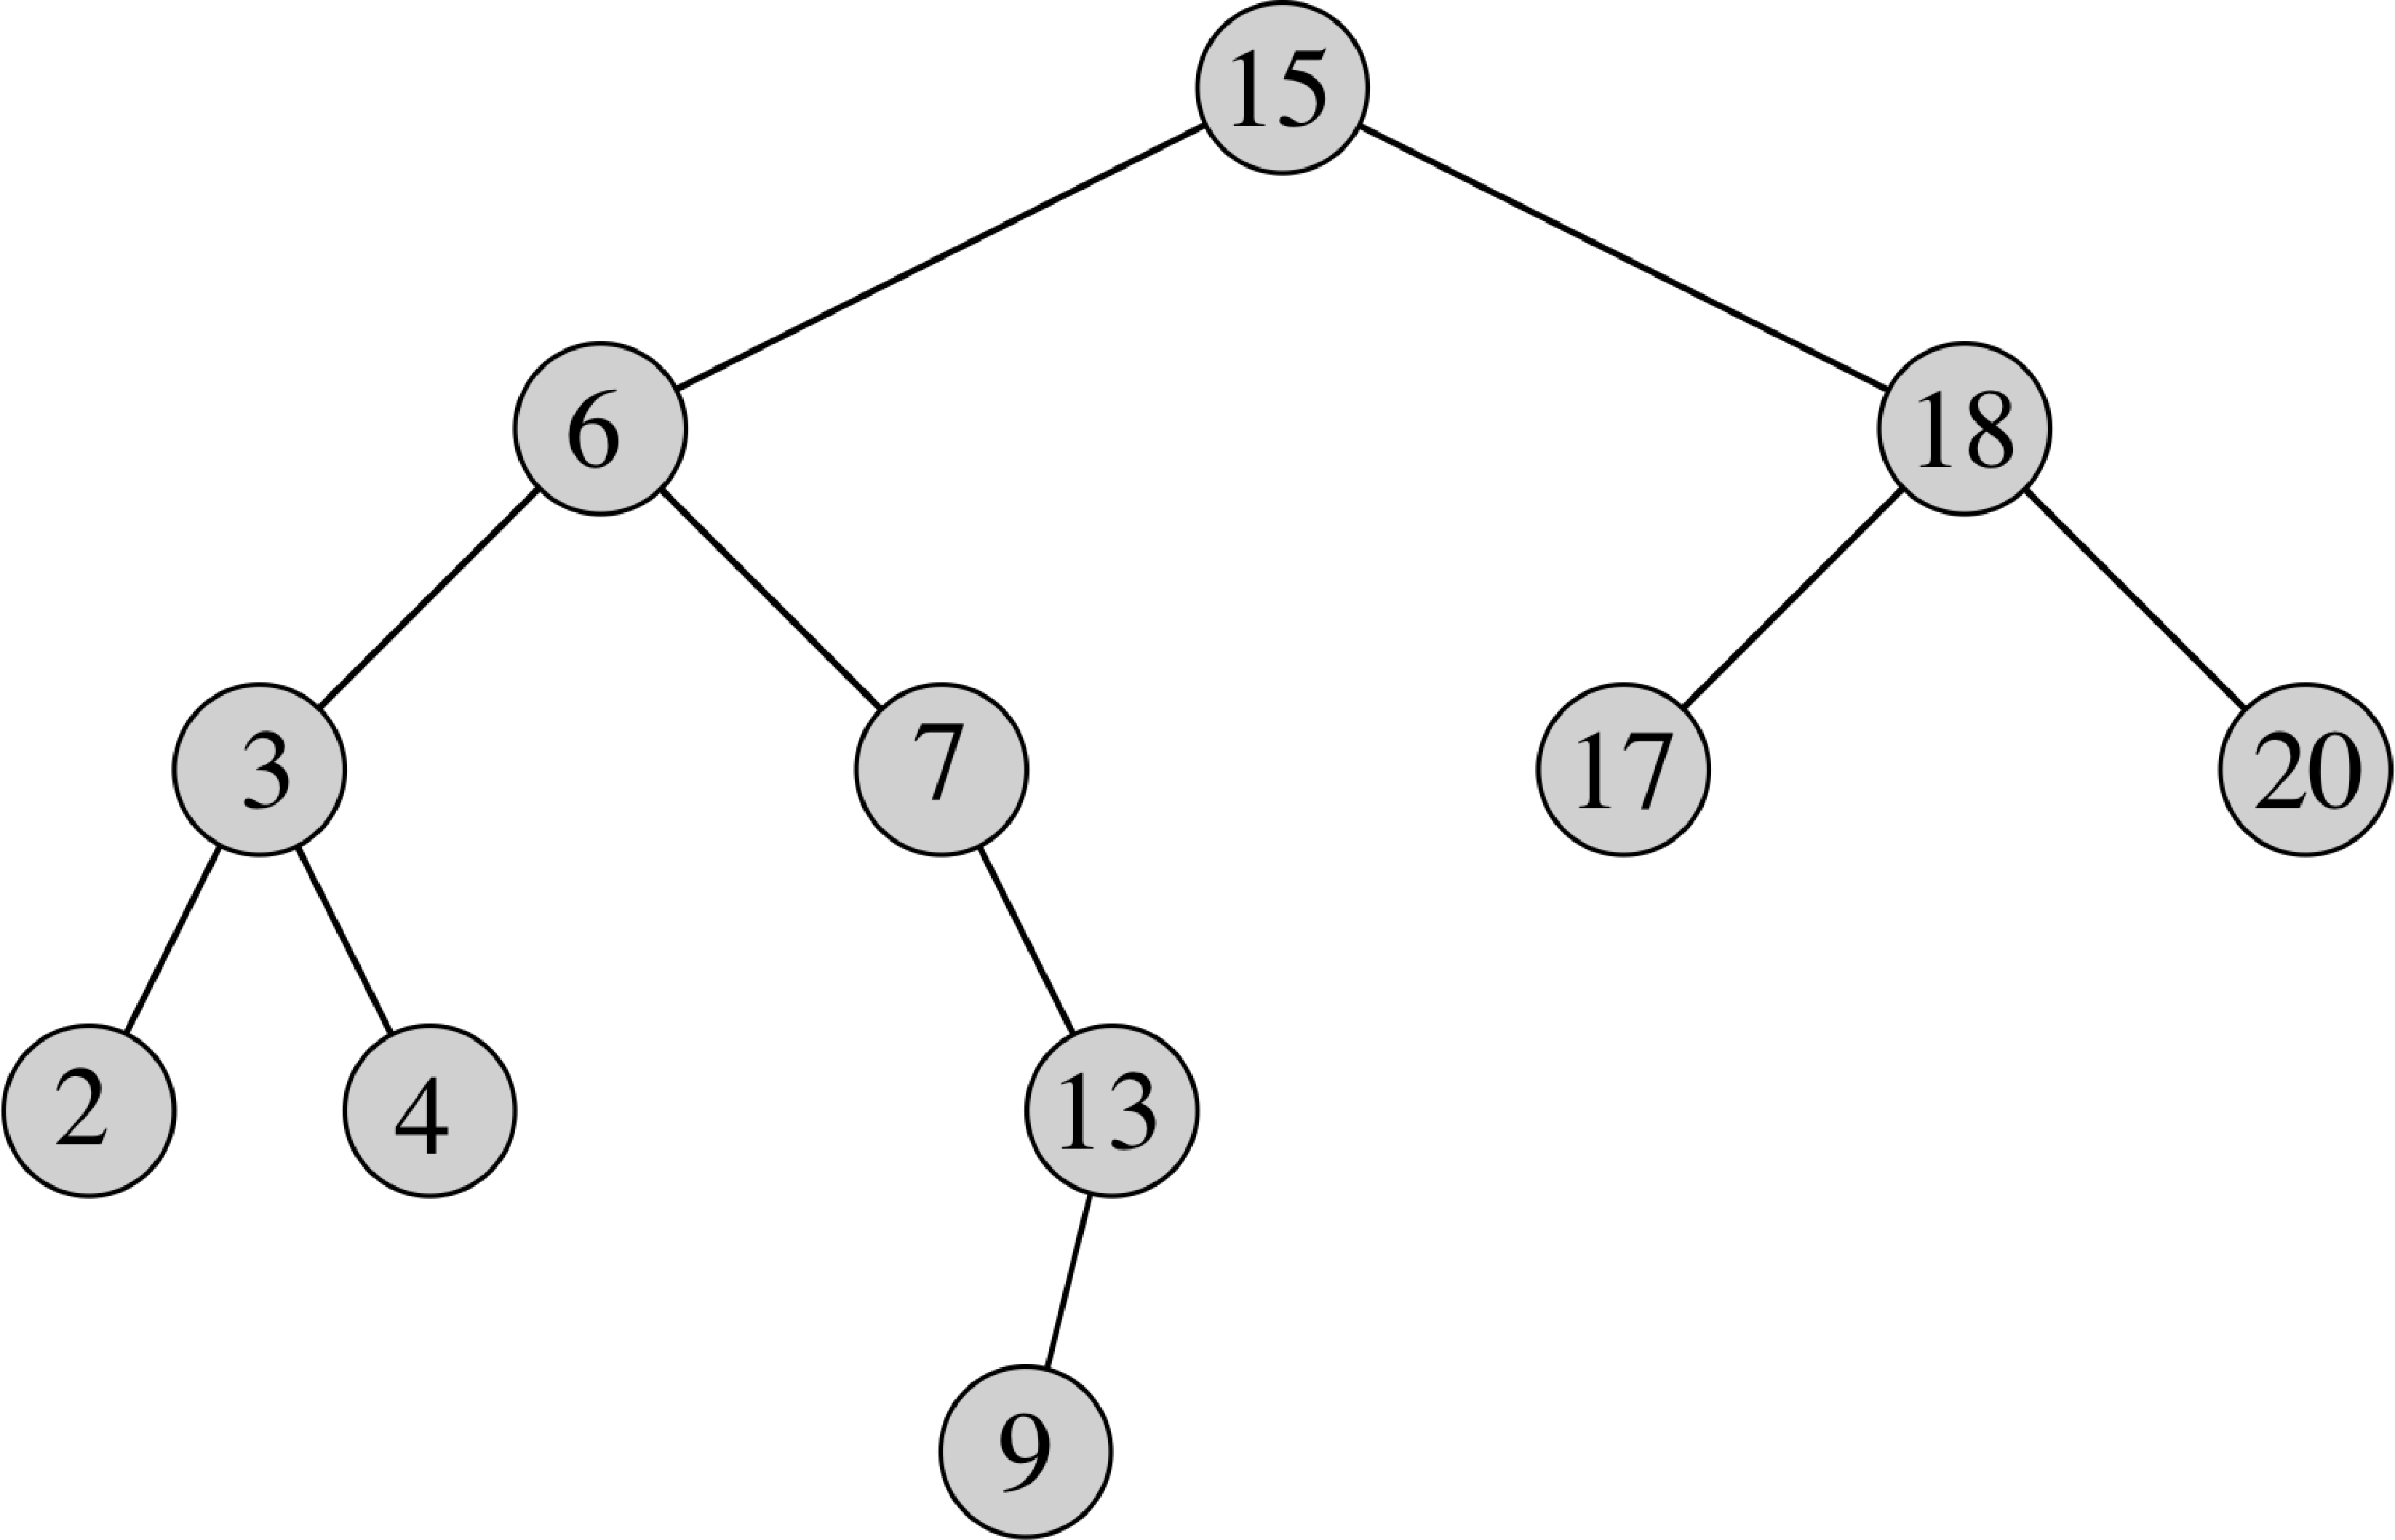
\includegraphics[width=0.5\textwidth]{Fig-12-2.pdf}

\bi
\ii Correctness follows from binary search tree property.
\ii Time:
$\Theta(n)$, because we visit and print each node once.
\bi\ii Formal proof
in book.\ei
\ei

\end{frame}
\sect{Tree-Search}
\begin{codebox}
  \Procname{$\proc{Tree-Search}(x,k)$}
  \li \If $x \isequal \const{nil}$ or $k\isequal\attrib{x}{key}$ \Do
  \li \Return $x$ \End
  \li \If $x < \attrib{x}{key}$ \Do
  \li \Return $\proc{Tree-Search}(\attrib{x}{left}, k)$ \End
  \li \Else \Return $\proc{Tree-Search}(\attrib{x}{right}, k)$ \End
\end{codebox}

\begin{multicols}{2}
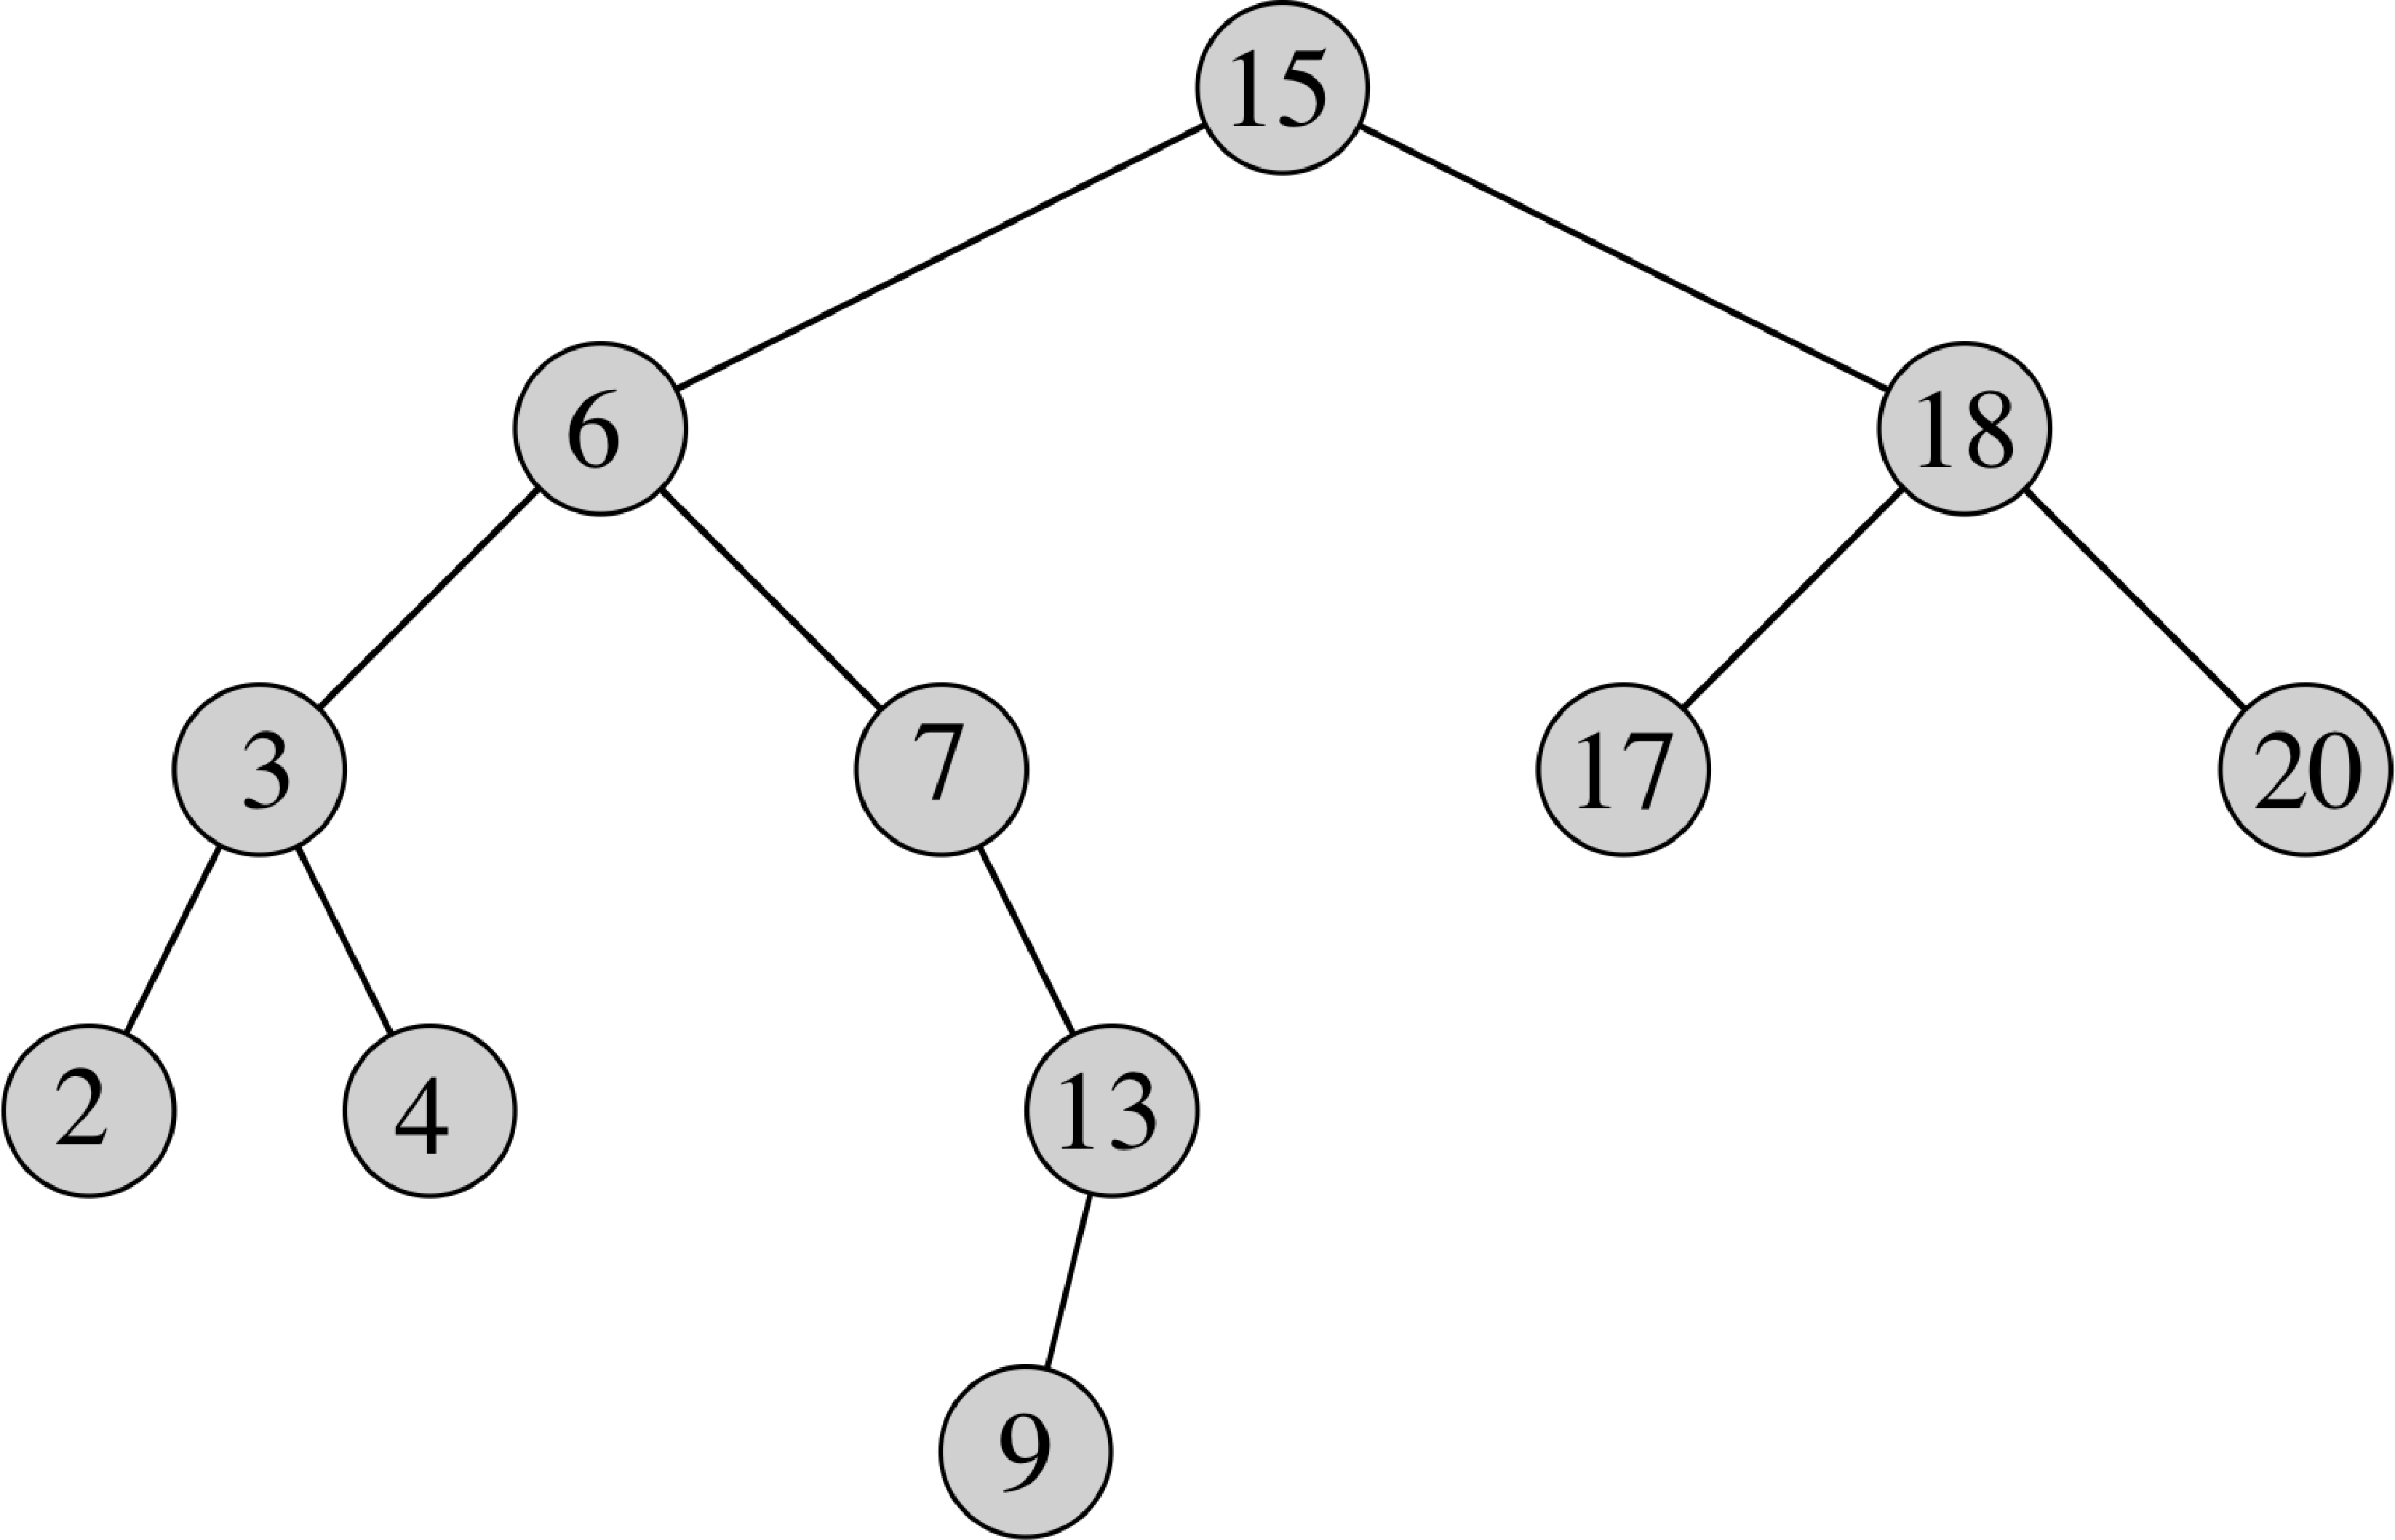
\includegraphics[width=0.5\textwidth]{Fig-12-2.pdf}

\bi
\ii The algorithm has a single recursion on a downward path from the
root.
\ii Time: $O(h)$ where $h$ is the height of the tree.
\ei
\end{multicols}

\end{frame}

\sect{Iterative version}


\begin{codebox}
  \Procname{$\proc{Tree-Search}(x,k)$}
  \li \If $x \isequal \const{nil}$ or $k\isequal\attrib{x}{key}$ \Do
  \li \Return $x$ \End
  \li \If $x < \attrib{x}{key}$ \Do
  \li \Return $\proc{Tree-Search}(\attrib{x}{left}, k)$ \End
  \li \Else \Return $\proc{Tree-Search}(\attrib{x}{right}, k)$ \End
\end{codebox}

\vfill

\begin{codebox}
  \Procname{$\proc{Iterative-Tree-Search}(x,k)$}
  \li \While $x \not\isequal \const{nil}$ and $k\not\isequal\attrib{x}{key}$ \Do
  \li \If $x < \attrib{x}{key}$ \Do
  \li $x\gets\attrib{x}{left}$ 
  \li \Else $x\gets\attrib{x}{right} $\End\End
  \li \Return $x$
\end{codebox}

\vfill

\bi\ii Tail recursion is easy to eliminate.\ei

\end{frame}

\sect{Minimum and maximum}
\footnotesize

\begin{multicols}{2}
\begin{codebox}
  \Procname{$\proc{Tree-Minimum}(x)$}
  \li \While $\attrib{x}{left} \not\isequal \const{nil}$ \Do
  \li $x\gets\attrib{x}{left}$ \End
  \li \Return $x$
\end{codebox}
\columnbreak
\begin{codebox}
  \Procname{$\proc{Tree-Minimum-Rec}(x)$}
  \li \If $\attrib{x}{left} \isequal \const{nil}$ \Do
  \li \Return $x$\End
  \li \Return $\proc{Tree-Minimum-Rec}(\attrib{x}{left})$
\end{codebox}
\end{multicols}

\vfill

\begin{multicols}{2}
\begin{codebox}
  \Procname{$\proc{Tree-Maximum}(x)$}
  \li \While $\attrib{x}{right} \not\isequal \const{nil}$ \Do
  \li $x\gets\attrib{x}{right}$ \End
  \li \Return $x$
\end{codebox}
\columnbreak
\begin{codebox}
  \Procname{$\proc{Tree-Maximum-Rec}(x)$}
  \li \If $\attrib{x}{right} \isequal \const{nil}$ \Do
  \li \Return $x$\End
  \li \Return $\proc{Tree-Minimum-Rec}(\attrib{x}{right})$
\end{codebox}
\end{multicols}

\vfill
\bi
\ii Both procedures trace a path from root to leaf.
\ii $O(h)$
\ei


\end{frame}

\sect{Successor and predecessor}
\footnotesize
\bi
\ii Assume all keys are distinct.
\ii The successor of a node $x$
is the node $y$ such that
\bi\ii$\attrib{y}{key}$ is the smallest key
$>\attrib{x}{key}$.\ei
\ii We can find successor without looking at keys.
\ii If $x$ has the largest key, its successor is $\const{nil}$.
\ii Two cases:
\begin{enumerate}
\item If node $x$ has a non-empty right subtree, return its minimum.
\item Otherwise,
 move up the tree until the first right turn.
\end{enumerate}
\ei
\begin{multicols}{2}
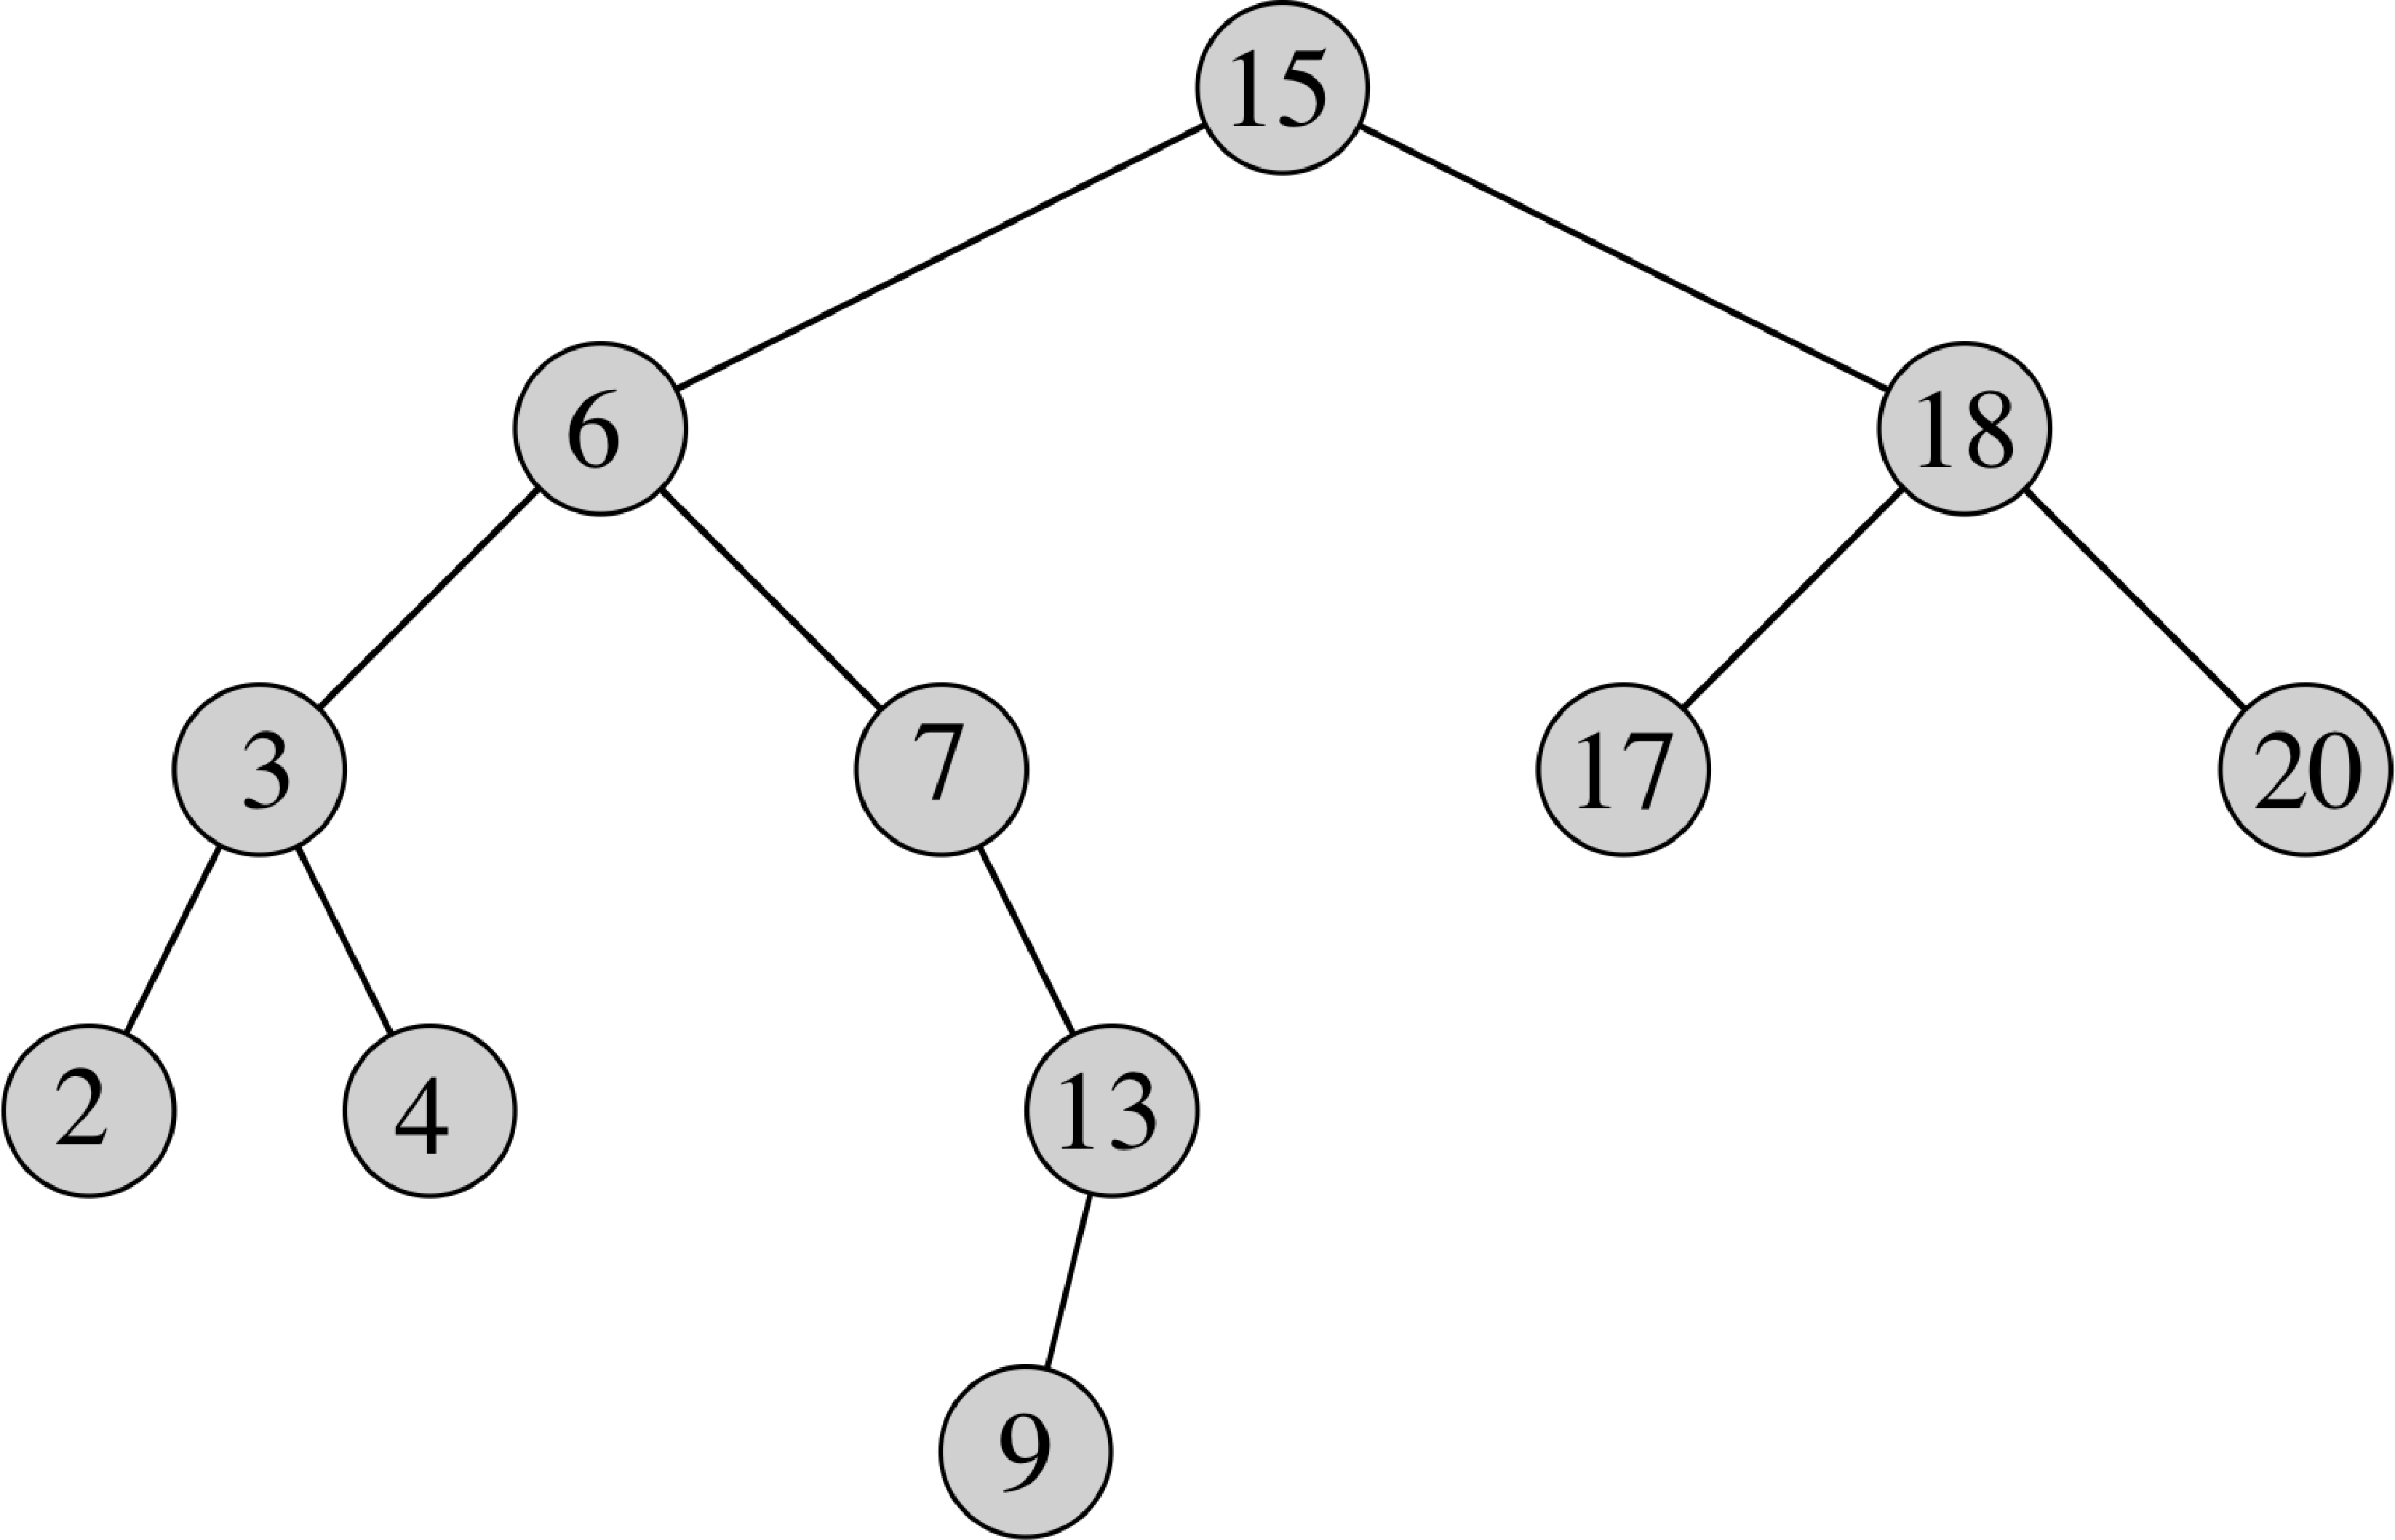
\includegraphics[width=0.45\textwidth]{Fig-12-2.pdf}

  \begin{codebox}
  \Procname{$\proc{Tree-Successor}(x)$}
  \li \If $\attrib{x}{right} \not\isequal \const{nil}$ \Do
  \li \Return $\proc{Tree-Minimum}(\attrib{x}{right})$ \End
  \li $y\gets\attrib{x}{p}$ 
  \li \While $y\not\isequal\const{nil}$ and
  $x\isequal\attrib{y}{right}$\Do
  \li $x\gets y$
  \li $y\gets \attrib{y}{p}$\End
  \li \Return $y$
\end{codebox}

\end{multicols}


\vfill

\bi
\ii Can also move up until parent key $\geq$ child key, but that uses keys.
\ii \textsc{Tree-Predecessor} similar.  Both are $O(h)$.
\ei

\begin{minipage}{0.5\textwidth}
\begin{codebox}
  \Procname{$\proc{Tree-Insert}(T,z)$}
  \li $y\gets \const{nil}$
  \li $x\gets \attrib{T}{root}$
  \li \While $x\not\isequal\const{nil}$\Do
  \li $y\gets x$
  \li \If $\attrib{z}{key} < \attrib{x}{key} $\Do
  \li $x\gets \attrib{x}{left}$ 
  \li \Else $x\gets \attrib{x}{right}$ \End\End
  \li $\attrib{z}{p} \gets y$
  \li \If $y\isequal\const{nil}$\Do
  \li $\attrib{T}{root}\gets z$
  \li \ElseIf $\attrib{z}{key} < \attrib{y}{key}$\Do
  \li $\attrib{y}{left}\gets z$
  \li \Else $\attrib{y}{right}\gets z$
  \End
\end{codebox}
\end{minipage}
\begin{minipage}{0.5\textwidth}
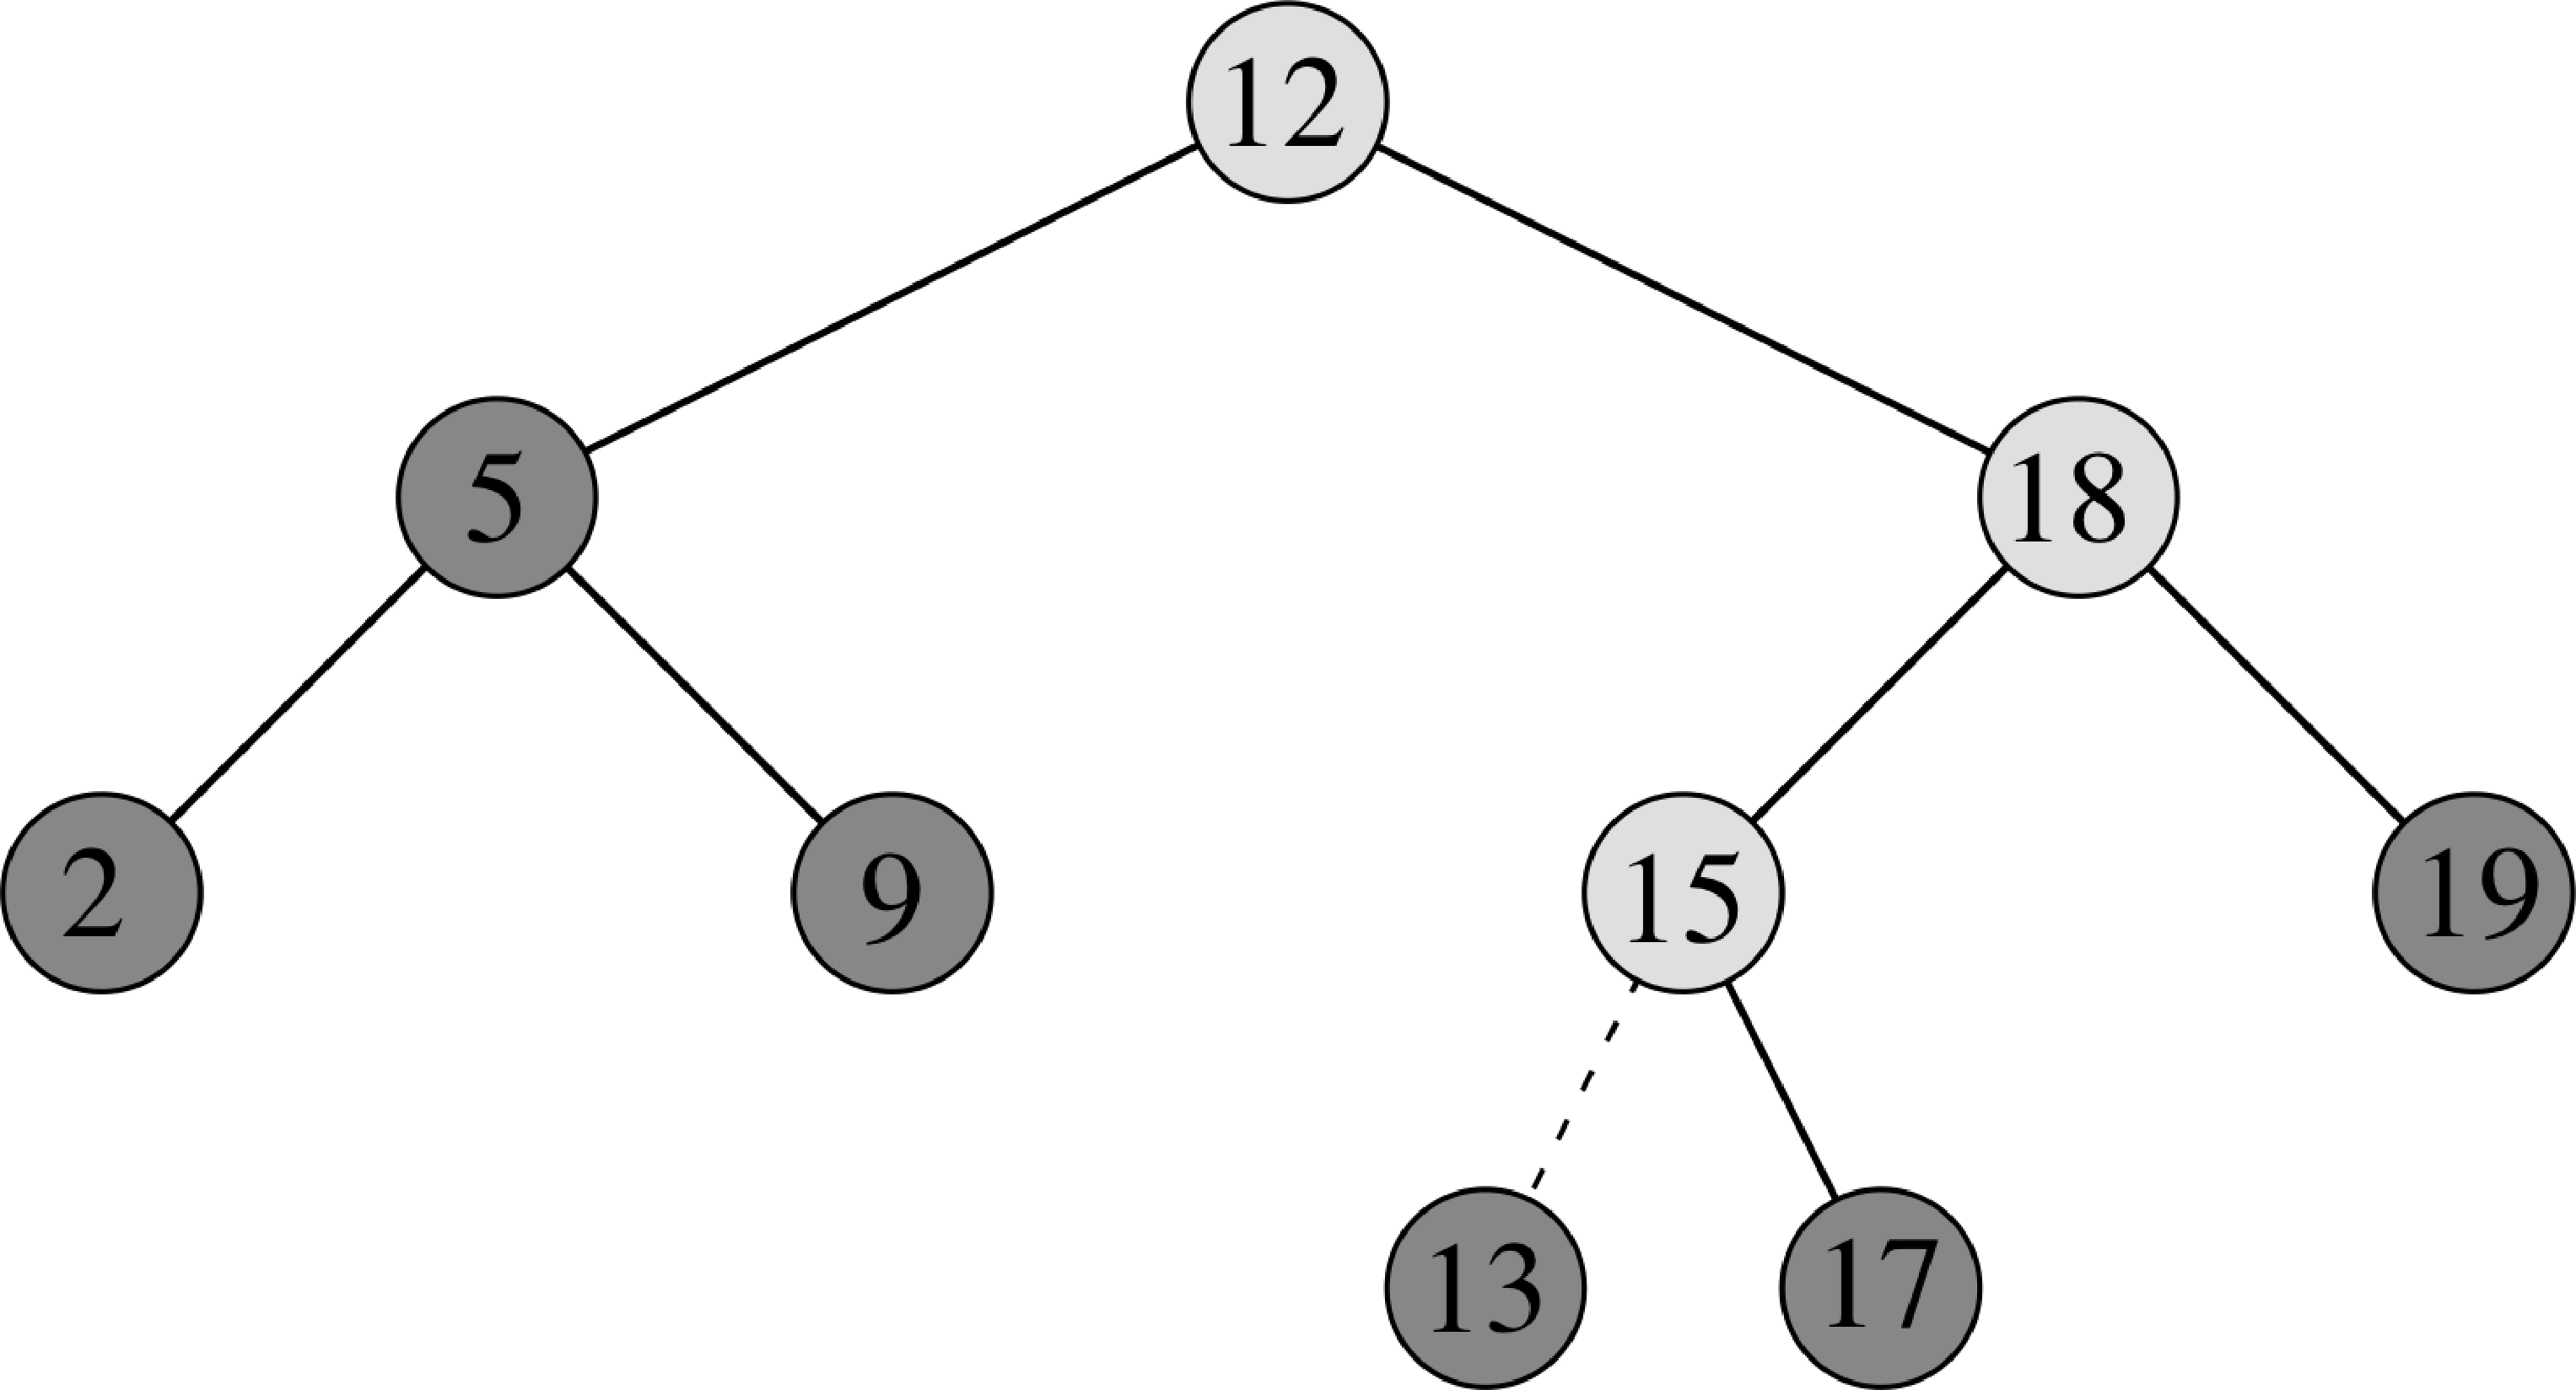
\includegraphics[width=\textwidth]{Fig-12-3.pdf}
\end{minipage}

\bi
\ii $O(h)$
\ii \textsc{Tree-Insert} can be used with \textsc{Inorder-Tree-Walk}
to sort.
\ei

\end{frame}

\sect{Tree insert}
\begin{multicols}{2}
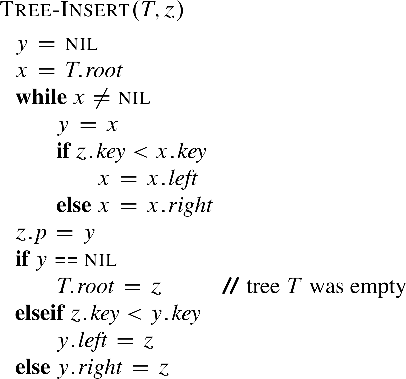
\includegraphics{Tree-Insert}

\mbox{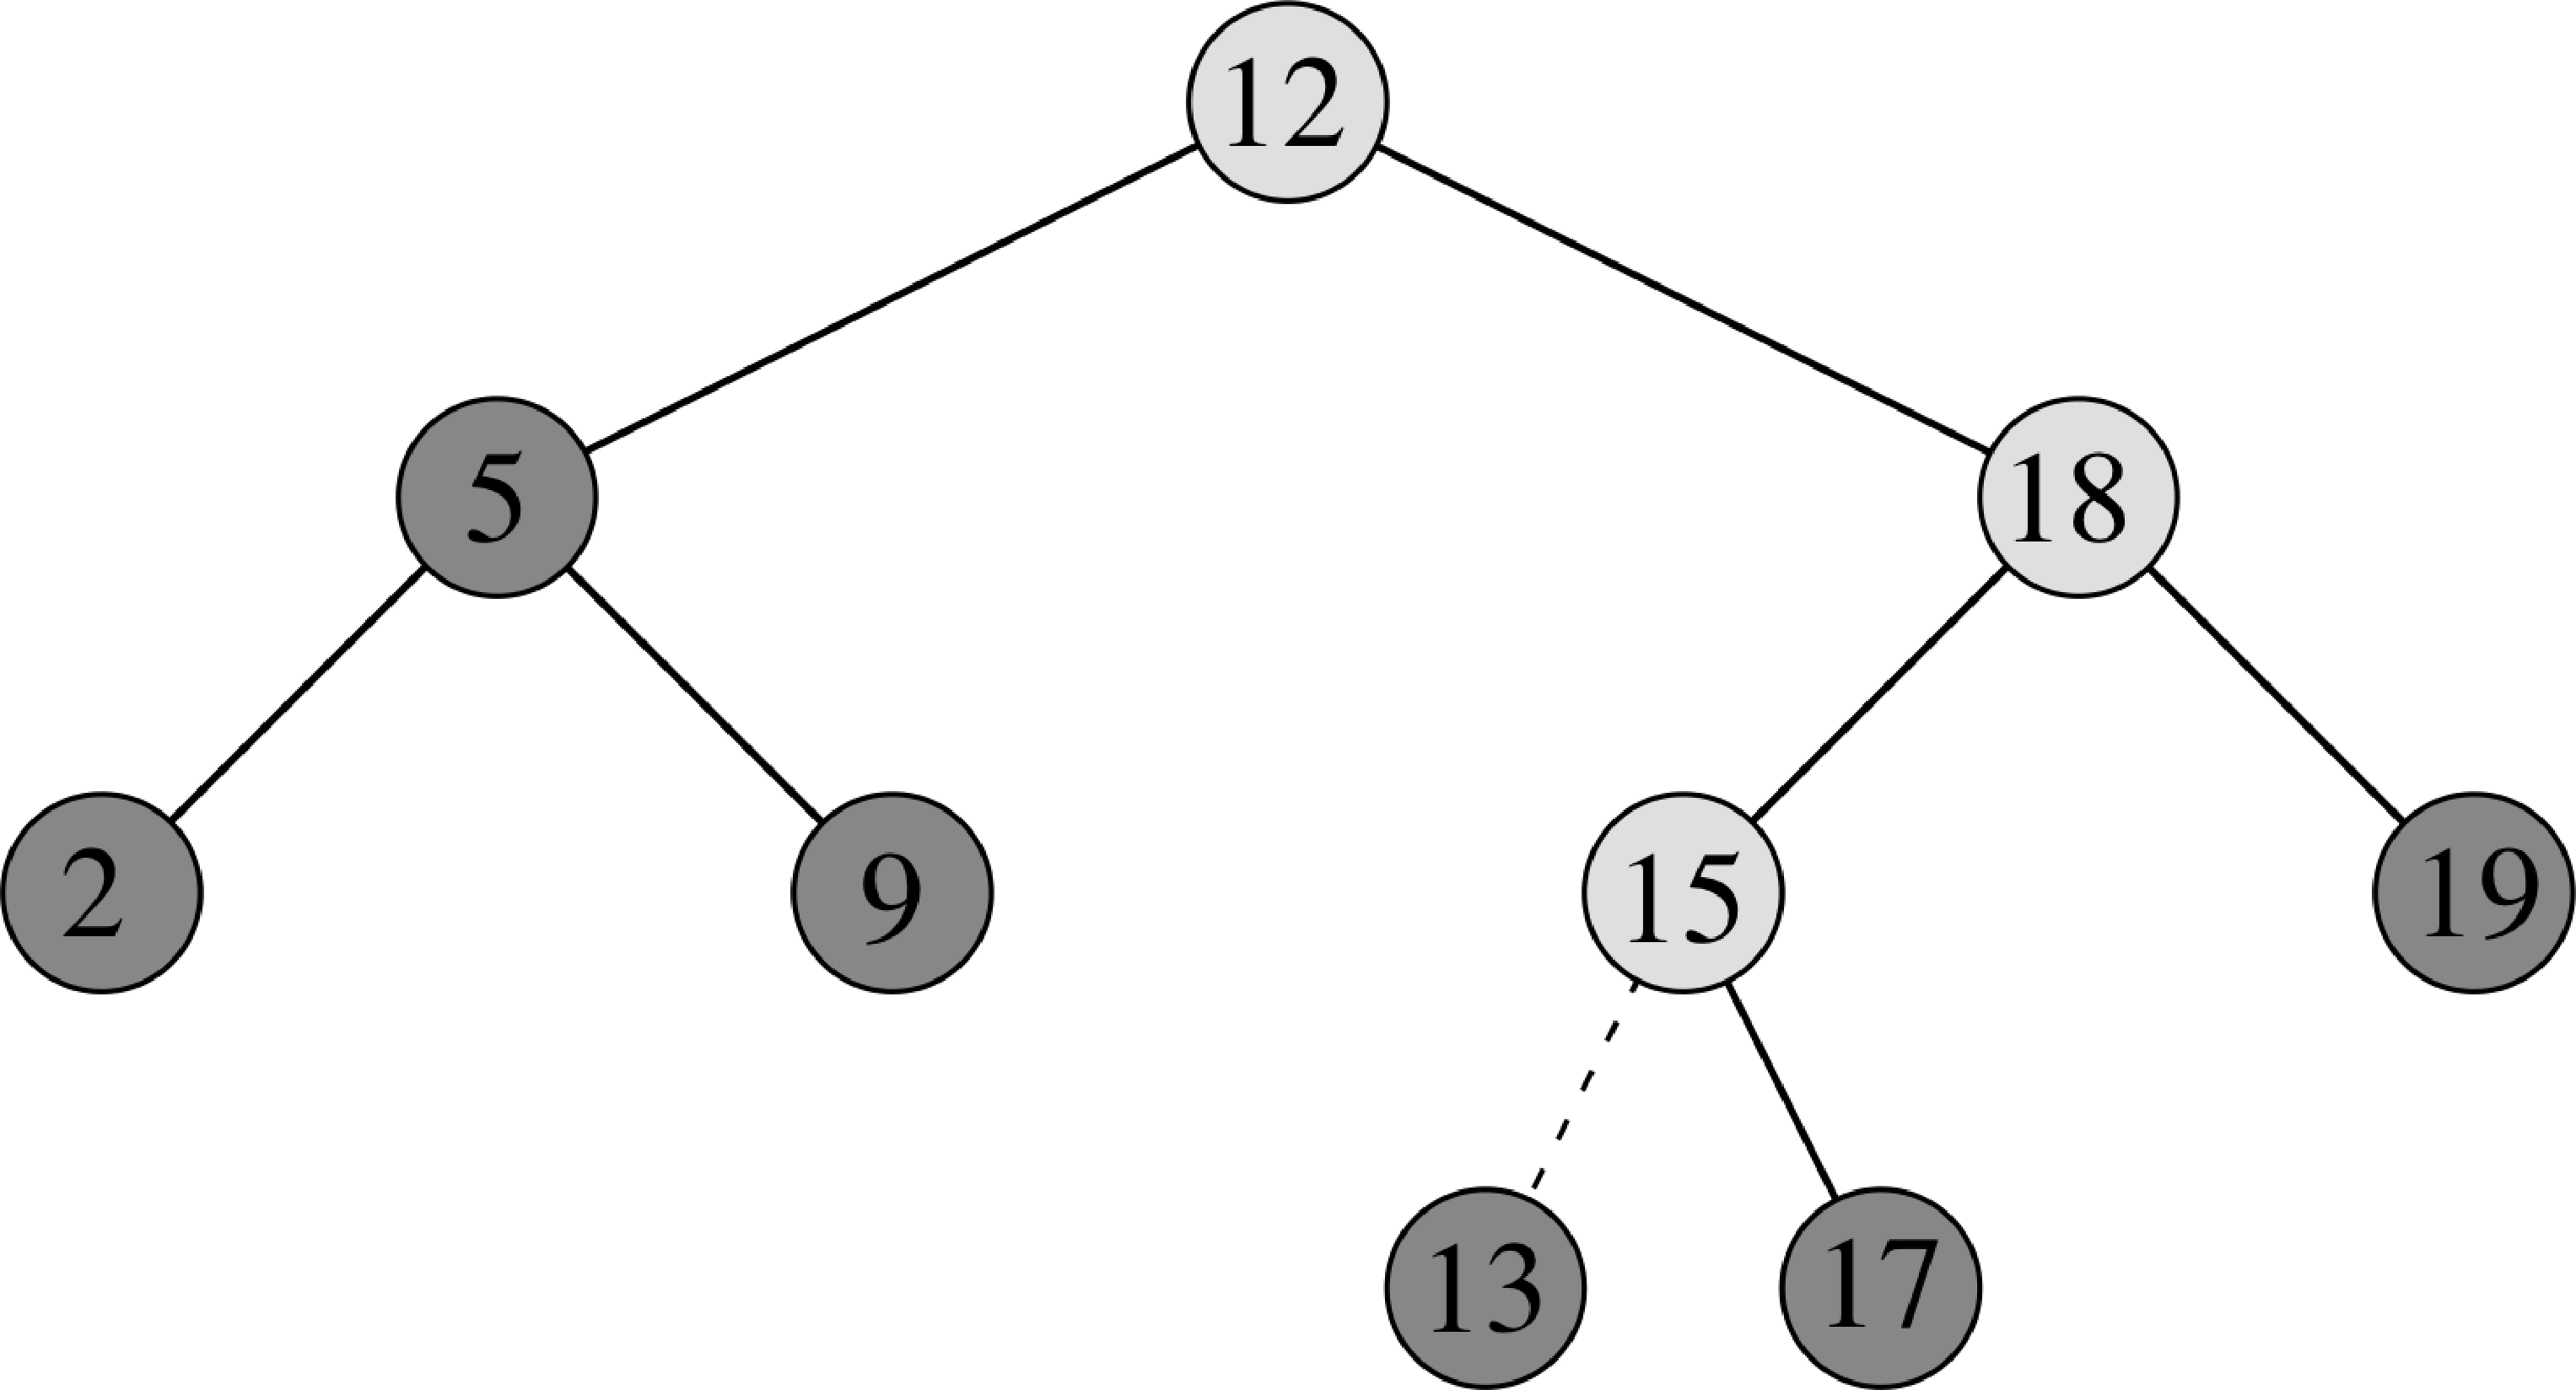
\includegraphics[width=0.5\textwidth]{Fig-12-3.pdf}}

\bi
\ii Trace downward path, maintaining parent pointer.
\ii Don't need parent pointer if we use a ``null structure''
for empty leaves.
\ei
\end{multicols}
\end{frame}

\sect{Recursive tree insert}
\footnotesize
\begin{multicols}{2}
\begin{codebox}
  \Procname{$\proc{Tree-Insert-Rec}(T,z)$}
  \li $\attrib{T}{root} \gets \proc{Node-Insert}(\attrib{T}{root}, z)$
\end{codebox}
\begin{codebox}
  \Procname{$\proc{Node-Insert}(x,z)$}
  \li \If $x\isequal\const{nil}$\Do
  \li \Return $z$\End
  \li $\attrib{z}{p}\gets x$
  \li \If $\attrib{z}{key} < \attrib{x}{key}$ \Do
  \li $\attrib{x}{left} \gets \proc{Node-Insert}(\attrib{x}{left}, z)$
  \li \Else
  \li $\attrib{x}{right} \gets \proc{Node-Insert}(\attrib{x}{right}, z)$
\End
\li \Return $x$
\end{codebox}

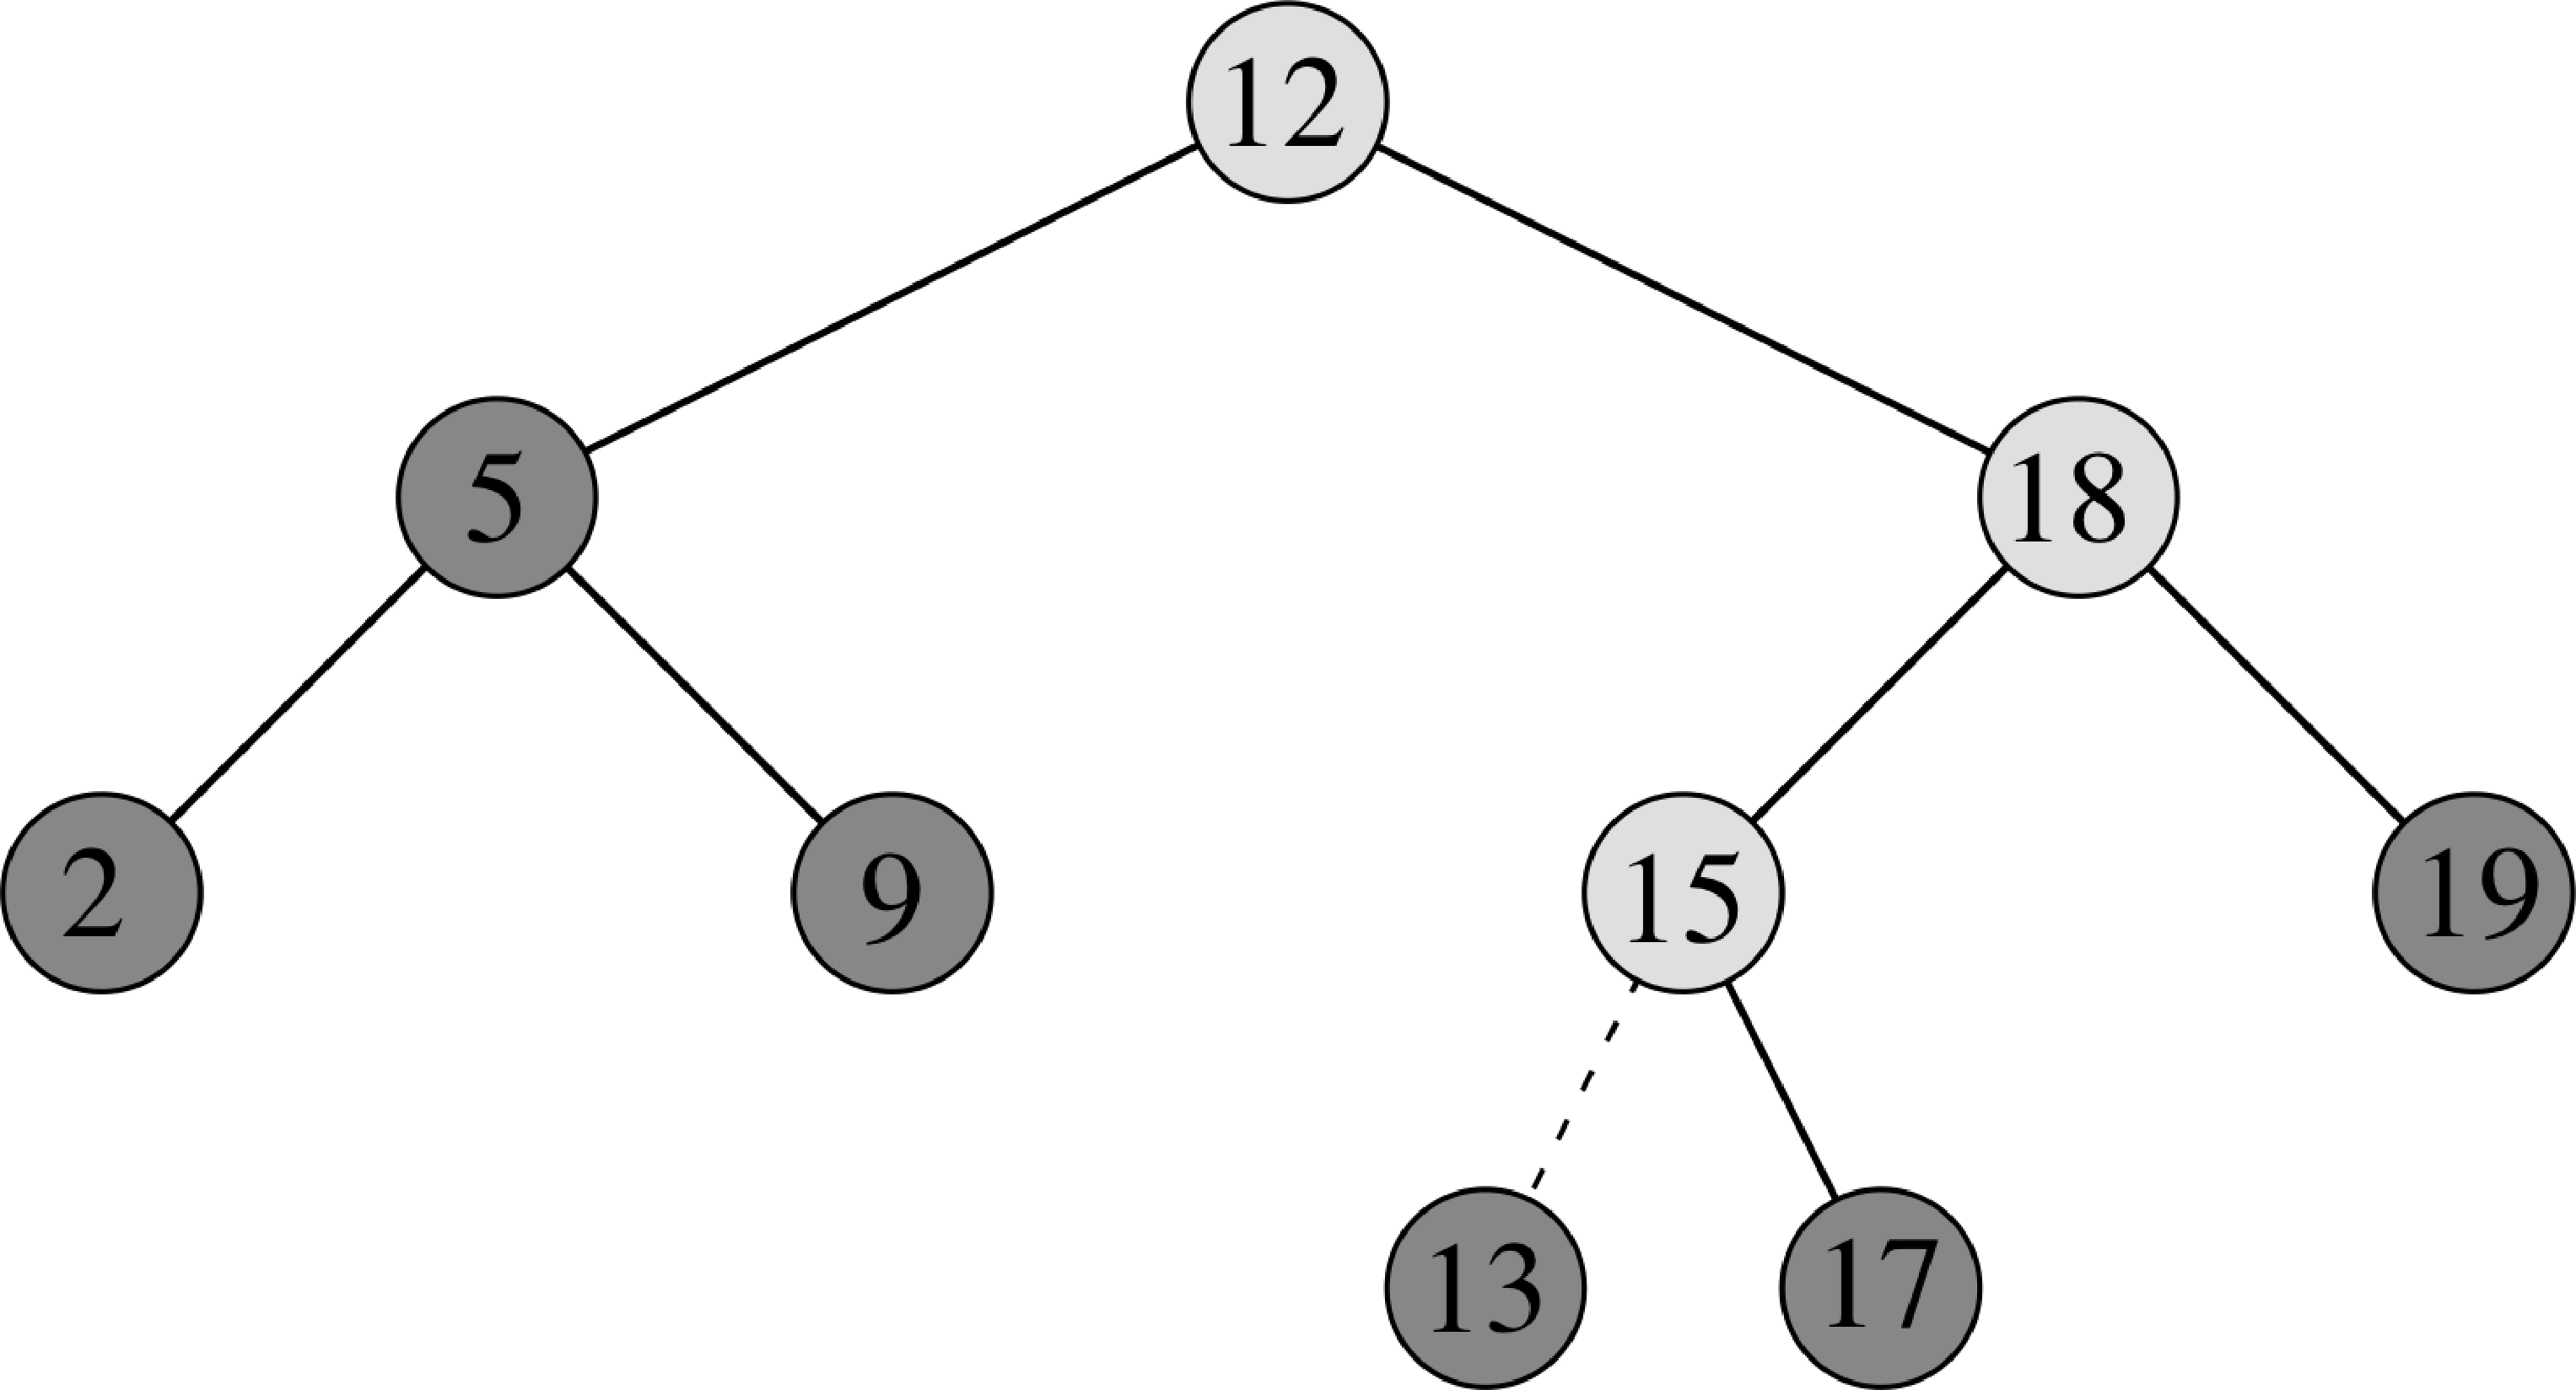
\includegraphics[width=0.5\textwidth]{Fig-12-3.pdf}
\end{multicols}
\end{frame}

\sect{Deletion}
\begin{multicols}{2}
  \scriptsize
To delete node $z$ from tree $T$:

(a) If $z$ has no children, just remove it.

(b) If $z$ has just one child, then make that child take $z$'s
  position in the tree.

(c) If $z$ has two children, then
  \bi
  \ii Find $z$'s successor $y$.
  \ii $y$ must be in $z$'s right subtree and have no left child.
  \ii $\attrib{y}{key}$ must be the smallest key in $z$'s right
  subtree.
  \ii $y$ can therefore replace $z$ at $z$'s position in the tree.
  \ii Deleting $y$'s node from the tree is easy because it has only
  one child.
  \ii $z$'s right subtree (now without $y$) becomes $y$'s right subtree.
  \ii $z$'s left child becomes $y$'s left child.
  \ei

\columnbreak

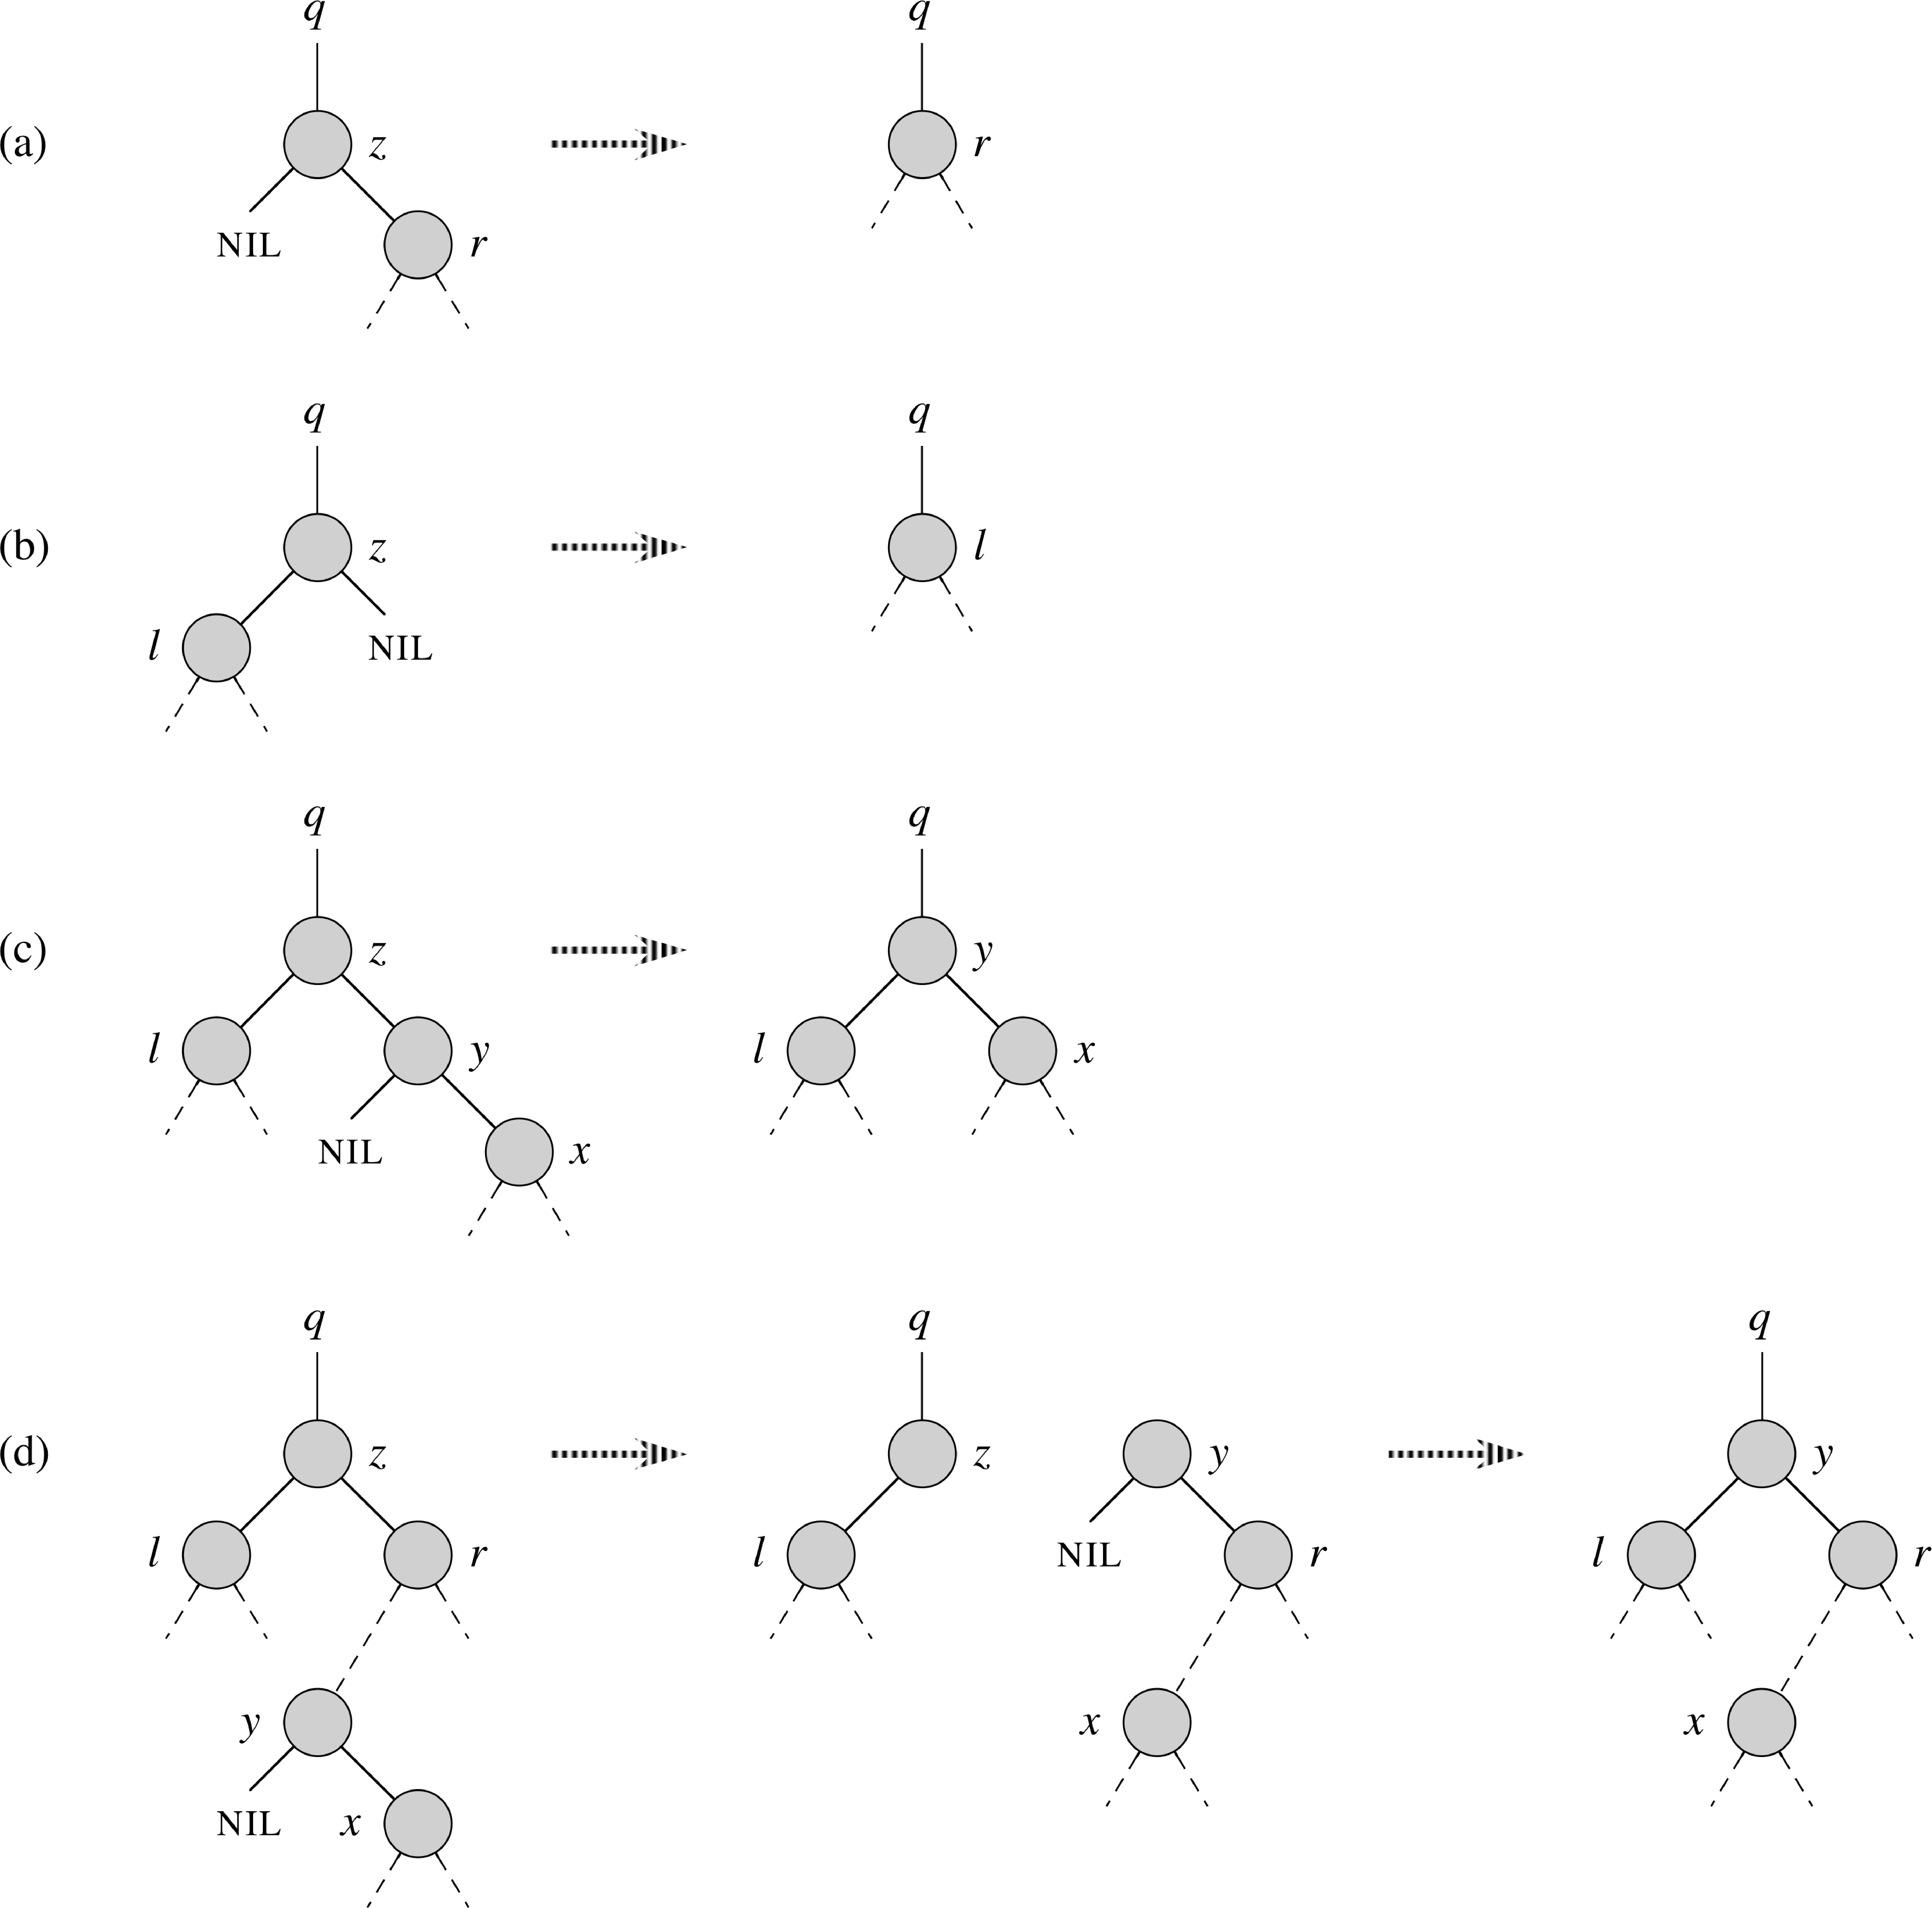
\includegraphics[height=0.6\textheight]{Fig-12-4.pdf}
\end{multicols}

\end{frame}

\sect{{\sc Transplant} and {\sc Tree-Delete}}
\footnotesize


\textsc{Transplant}$(T,u,v)$ replaces the subtree at $u$
with the subtree at $v$.

\begin{multicols}{2}
  
\begin{codebox}
  \Procname{$\proc{Transplant}(T,u,v)$}
    \li\If $\attrib{u}{p} \isequal \const{nil}$ \Do
    \li $\attrib{T}{root} \gets v$ 
    \li \ElseIf $u\isequal \attrib{\attrib{u}{p}}{left}$ \Do
    \li $\attrib{\attrib{u}{p}}{left} \gets v$ 
    \li \Else  $\attrib{\attrib{u}{p}}{right} \gets v$ \End
    \li \If $v\not\isequal\const{nil}$\Do
    \li $\attrib{v}{p}\gets\attrib{u}{p}$
    \End
\end{codebox}

\columnbreak

\begin{codebox}
  \Procname{$\proc{Tree-Delete}(T,z)$}
  \li\If $\attrib{z}{left}\isequal\const{nil}$  \Do
  \li $\proc{Transplant}(T,z,\attrib{z}{right})$ 
  \li \ElseIf $\attrib{z}{right} \isequal \const{nil}$ \Do
  \li $\proc{Transplant}(T,z,\attrib{z}{left})$
  \li \Else 
  \li $y\gets \proc{Tree-Minimum}(\attrib{z}{right})$
  \li \If $\attrib{y}{p} \not\isequal z$ \Do
  \li $\proc{Transplant}(T,y,\attrib{y}{right})$
  \li $\attrib{y}{right}\gets\attrib{z}{right}$
  \li $\attrib{\attrib{y}{right}}{p} \gets y$\End
  \li $\proc{Transplant}(T,z,y)$
  \li $\attrib{y}{left}\gets\attrib{z}{left}$
  \li $\attrib{\attrib{y}{left}}{p} \gets y$
  \End
\end{codebox}

\end{multicols}

\vfill

\bi\ii$O(h)$\ei



\end{frame}

\sect{Theorem 12.4}

The expected height of a randomly built binary search tree on
$n$ distinct keys is $O(\lg n)$.

\vfill
Proof in text.

\vfill

\bi
\ii Red-black trees and B-trees actively maintain a $O(\lg n)$ height
in worst case.
\ei

\vfill

\end{frame}

\sect{Problem 12-2, Radix trees}

$\{0,011,100,10,1011\}$

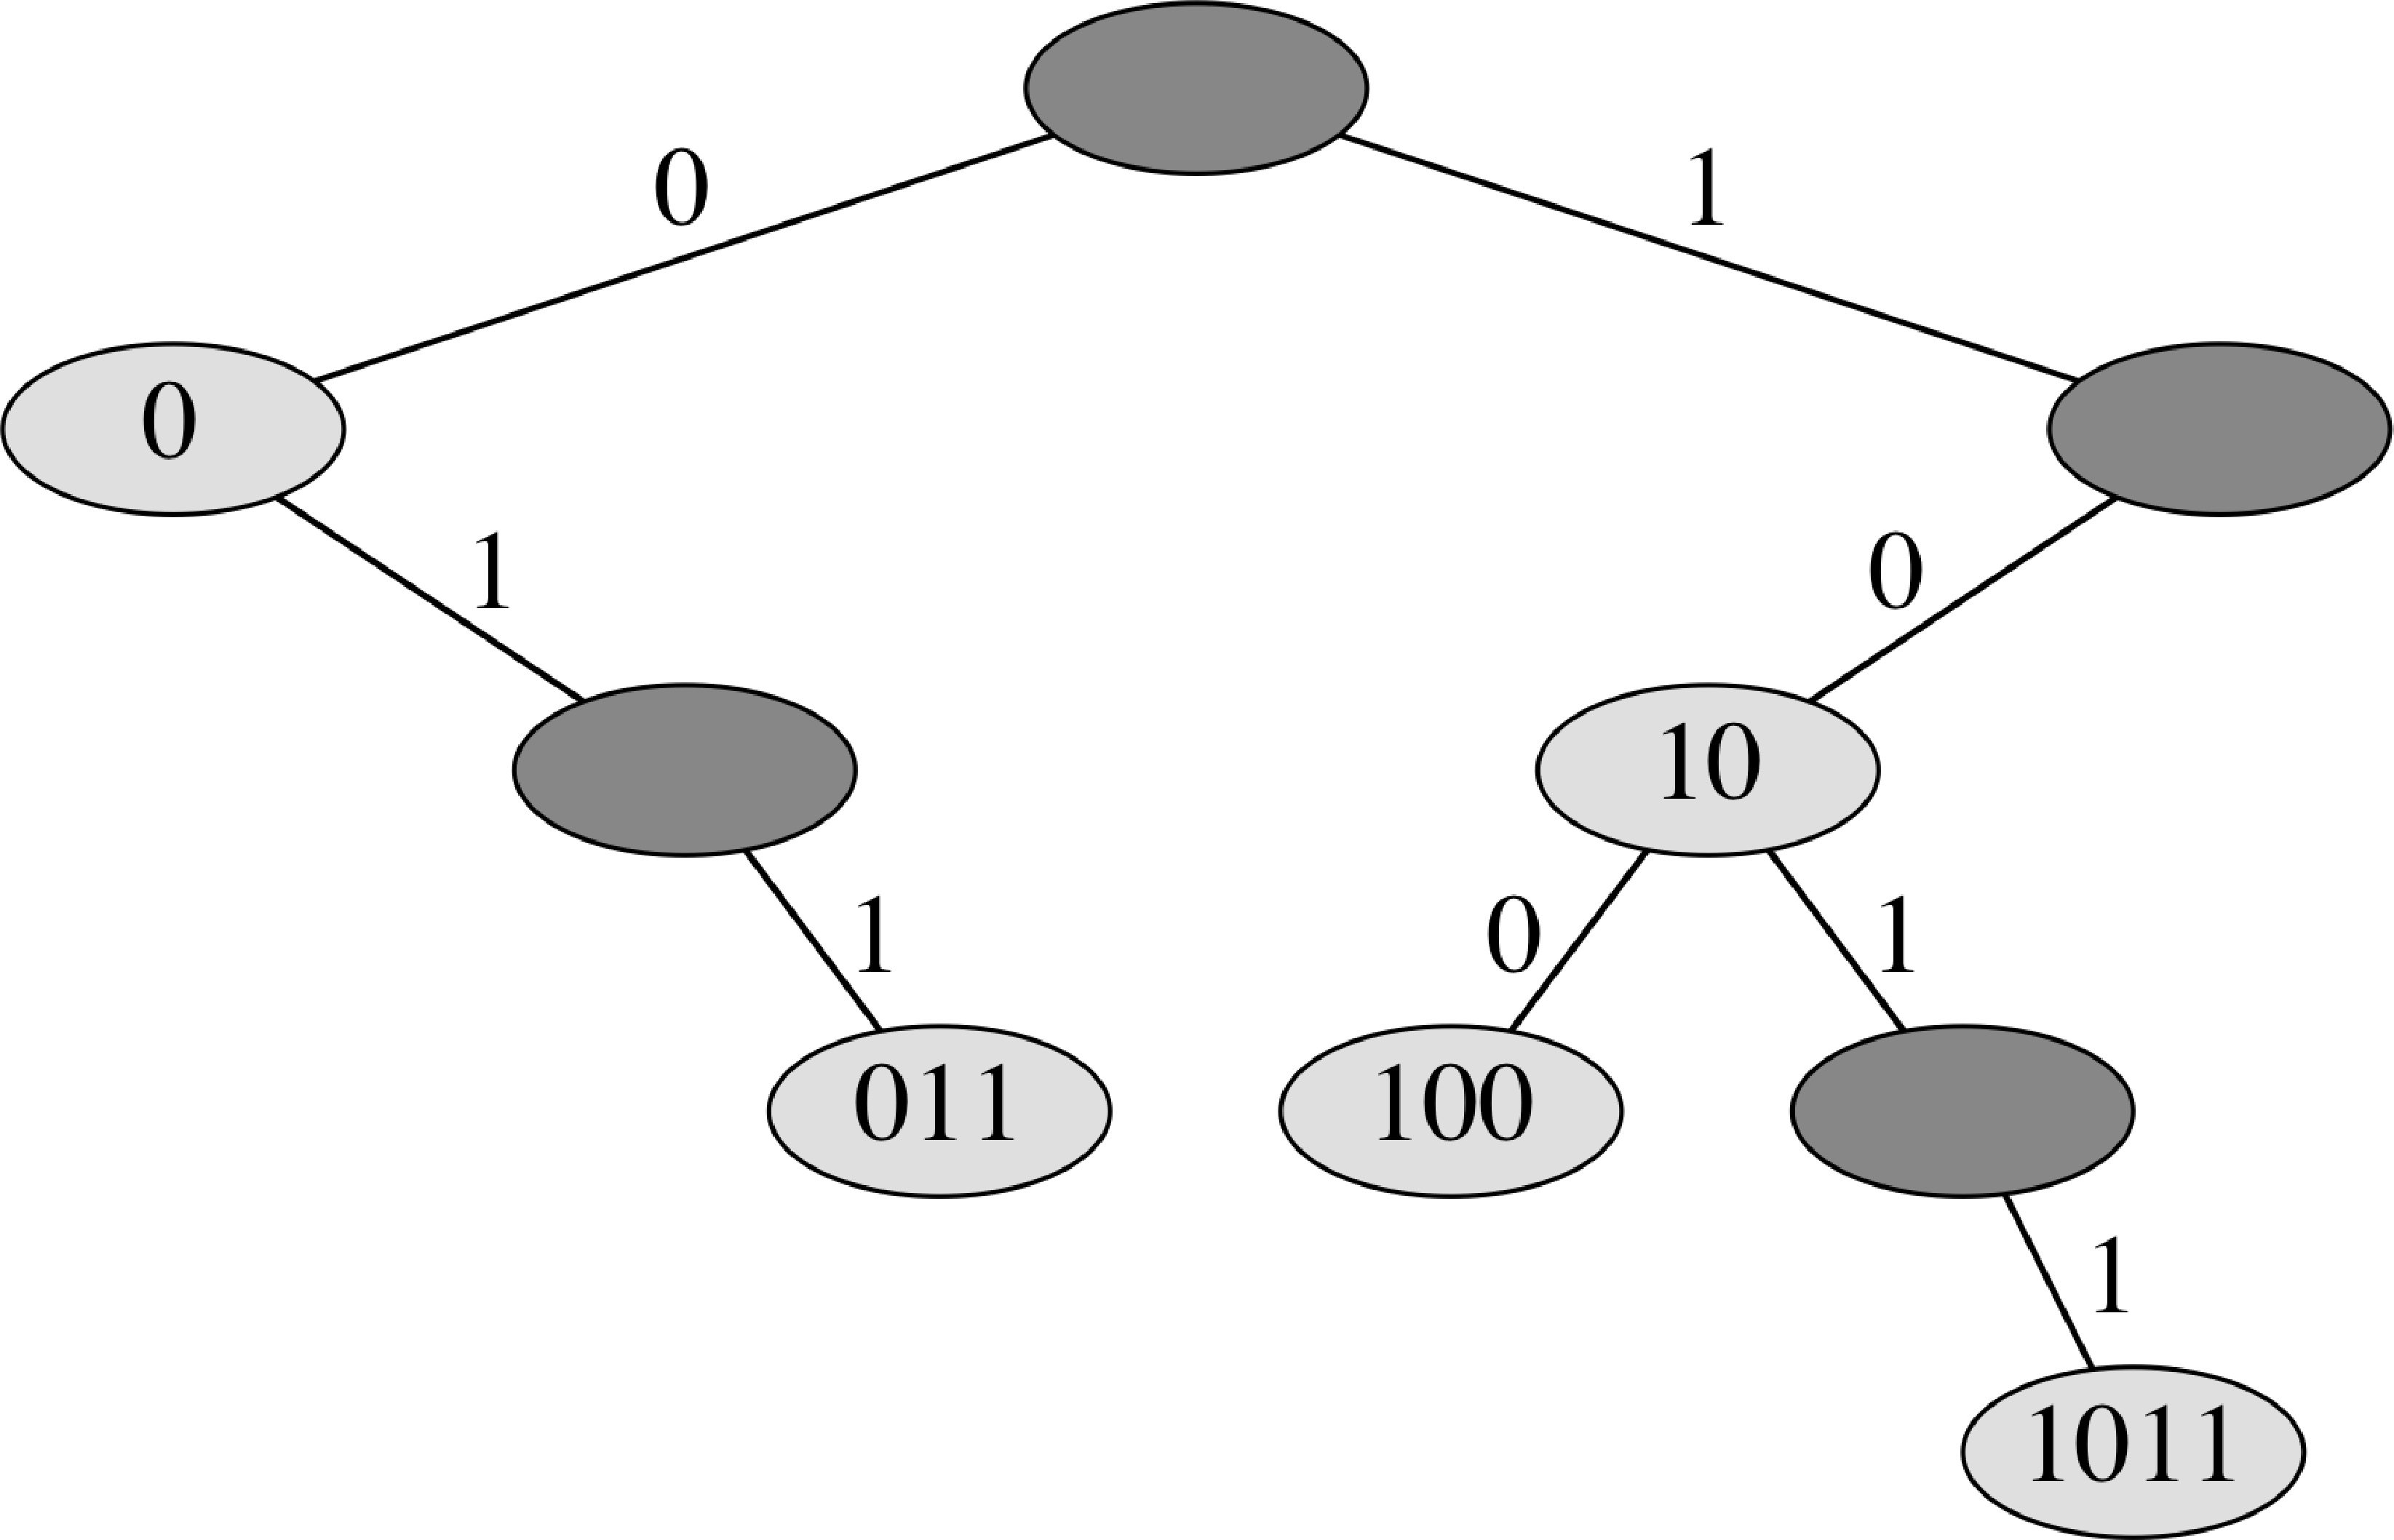
\includegraphics[width=0.5\textwidth]{Fig-12-5.pdf}


\bi
\ii $a=a_0a_1\ldots a_p$ is \textbf{lexicographically less than}
$b=b_0b_1\ldots b_q$: 
  \begin{enumerate}
  \item
    there exists and integer $j$, where $0\leq j \leq\min(p,q)$,
  such that\\ $a_i=b_i$ for all $i=0,1,\ldots,j-1$ and $a_j<b_j$, or
\item
  $p<q$ and $a_i=b_i$ for all $i=0,1,\ldots,p$.
  \end{enumerate}

  \ii Show that
  a set $S$ of bit strings can be sorted lexicographically
in $\Theta(n)$ time,\\ where $n$ is the sum of the lengths of the
strings in $S$.
\ei

\end{frame}

\end{document}
